\documentclass[twoside]{book}

% Packages required by doxygen
\usepackage{fixltx2e}
\usepackage{calc}
\usepackage{doxygen}
\usepackage[export]{adjustbox} % also loads graphicx
\usepackage{graphicx}
\usepackage[utf8]{inputenc}
\usepackage{makeidx}
\usepackage{multicol}
\usepackage{multirow}
\PassOptionsToPackage{warn}{textcomp}
\usepackage{textcomp}
\usepackage[nointegrals]{wasysym}
\usepackage[table]{xcolor}

% Font selection
\usepackage[T1]{fontenc}
\usepackage[scaled=.90]{helvet}
\usepackage{courier}
\usepackage{amssymb}
\usepackage{sectsty}
\renewcommand{\familydefault}{\sfdefault}
\allsectionsfont{%
  \fontseries{bc}\selectfont%
  \color{darkgray}%
}
\renewcommand{\DoxyLabelFont}{%
  \fontseries{bc}\selectfont%
  \color{darkgray}%
}
\newcommand{\+}{\discretionary{\mbox{\scriptsize$\hookleftarrow$}}{}{}}

% Page & text layout
\usepackage{geometry}
\geometry{%
  a4paper,%
  top=2.5cm,%
  bottom=2.5cm,%
  left=2.5cm,%
  right=2.5cm%
}
\tolerance=750
\hfuzz=15pt
\hbadness=750
\setlength{\emergencystretch}{15pt}
\setlength{\parindent}{0cm}
\setlength{\parskip}{3ex plus 2ex minus 2ex}
\makeatletter
\renewcommand{\paragraph}{%
  \@startsection{paragraph}{4}{0ex}{-1.0ex}{1.0ex}{%
    \normalfont\normalsize\bfseries\SS@parafont%
  }%
}
\renewcommand{\subparagraph}{%
  \@startsection{subparagraph}{5}{0ex}{-1.0ex}{1.0ex}{%
    \normalfont\normalsize\bfseries\SS@subparafont%
  }%
}
\makeatother

% Headers & footers
\usepackage{fancyhdr}
\pagestyle{fancyplain}
\fancyhead[LE]{\fancyplain{}{\bfseries\thepage}}
\fancyhead[CE]{\fancyplain{}{}}
\fancyhead[RE]{\fancyplain{}{\bfseries\leftmark}}
\fancyhead[LO]{\fancyplain{}{\bfseries\rightmark}}
\fancyhead[CO]{\fancyplain{}{}}
\fancyhead[RO]{\fancyplain{}{\bfseries\thepage}}
\fancyfoot[LE]{\fancyplain{}{}}
\fancyfoot[CE]{\fancyplain{}{}}
\fancyfoot[RE]{\fancyplain{}{\bfseries\scriptsize Generated by Doxygen }}
\fancyfoot[LO]{\fancyplain{}{\bfseries\scriptsize Generated by Doxygen }}
\fancyfoot[CO]{\fancyplain{}{}}
\fancyfoot[RO]{\fancyplain{}{}}
\renewcommand{\footrulewidth}{0.4pt}
\renewcommand{\chaptermark}[1]{%
  \markboth{#1}{}%
}
\renewcommand{\sectionmark}[1]{%
  \markright{\thesection\ #1}%
}

% Indices & bibliography
\usepackage{natbib}
\usepackage[titles]{tocloft}
\setcounter{tocdepth}{3}
\setcounter{secnumdepth}{5}
\makeindex

% Hyperlinks (required, but should be loaded last)
\usepackage{ifpdf}
\ifpdf
  \usepackage[pdftex,pagebackref=true]{hyperref}
\else
  \usepackage[ps2pdf,pagebackref=true]{hyperref}
\fi
\hypersetup{%
  colorlinks=true,%
  linkcolor=blue,%
  citecolor=blue,%
  unicode%
}

% Custom commands
\newcommand{\clearemptydoublepage}{%
  \newpage{\pagestyle{empty}\cleardoublepage}%
}

\usepackage{caption}
\captionsetup{labelsep=space,justification=centering,font={bf},singlelinecheck=off,skip=4pt,position=top}

%===== C O N T E N T S =====

\begin{document}

% Titlepage & ToC
\hypersetup{pageanchor=false,
             bookmarksnumbered=true,
             pdfencoding=unicode
            }
\pagenumbering{alph}
\begin{titlepage}
\vspace*{7cm}
\begin{center}%
{\Large Projeto 3° unidade }\\
\vspace*{1cm}
{\large Generated by Doxygen 1.8.14}\\
\end{center}
\end{titlepage}
\clearemptydoublepage
\pagenumbering{roman}
\tableofcontents
\clearemptydoublepage
\pagenumbering{arabic}
\hypersetup{pageanchor=true}

%--- Begin generated contents ---
\chapter{Hierarchical Index}
\section{Class Hierarchy}
This inheritance list is sorted roughly, but not completely, alphabetically\+:\begin{DoxyCompactList}
\item \contentsline{section}{Animal}{\pageref{classAnimal}}{}
\begin{DoxyCompactList}
\item \contentsline{section}{Anfibio}{\pageref{classAnfibio}}{}
\item \contentsline{section}{Ave}{\pageref{classAve}}{}
\begin{DoxyCompactList}
\item \contentsline{section}{Ave\+Exotica}{\pageref{classAveExotica}}{}
\item \contentsline{section}{Ave\+Nativa}{\pageref{classAveNativa}}{}
\end{DoxyCompactList}
\item \contentsline{section}{Mamifero}{\pageref{classMamifero}}{}
\item \contentsline{section}{Reptil}{\pageref{classReptil}}{}
\end{DoxyCompactList}
\item \contentsline{section}{Animal\+Silvestre}{\pageref{classAnimalSilvestre}}{}
\begin{DoxyCompactList}
\item \contentsline{section}{Exotico}{\pageref{classExotico}}{}
\begin{DoxyCompactList}
\item \contentsline{section}{Ave\+Exotica}{\pageref{classAveExotica}}{}
\end{DoxyCompactList}
\item \contentsline{section}{Nativo}{\pageref{classNativo}}{}
\begin{DoxyCompactList}
\item \contentsline{section}{Ave\+Nativa}{\pageref{classAveNativa}}{}
\end{DoxyCompactList}
\end{DoxyCompactList}
\item exception\begin{DoxyCompactList}
\item \contentsline{section}{Erro\+Ao\+Abrir\+Arquivo}{\pageref{classErroAoAbrirArquivo}}{}
\item \contentsline{section}{Erro\+Ao\+Tentar\+Ler\+Dados}{\pageref{classErroAoTentarLerDados}}{}
\end{DoxyCompactList}
\item \contentsline{section}{Funcionario}{\pageref{classFuncionario}}{}
\begin{DoxyCompactList}
\item \contentsline{section}{Tratador}{\pageref{classTratador}}{}
\item \contentsline{section}{Veterinario}{\pageref{classVeterinario}}{}
\end{DoxyCompactList}
\end{DoxyCompactList}

\chapter{Class Index}
\section{Class List}
Here are the classes, structs, unions and interfaces with brief descriptions\+:\begin{DoxyCompactList}
\item\contentsline{section}{\hyperlink{classAnfibio}{Anfibio} }{\pageref{classAnfibio}}{}
\item\contentsline{section}{\hyperlink{classAnimal}{Animal} }{\pageref{classAnimal}}{}
\item\contentsline{section}{\hyperlink{classAnimalSilvestre}{Animal\+Silvestre} }{\pageref{classAnimalSilvestre}}{}
\item\contentsline{section}{\hyperlink{classAve}{Ave} }{\pageref{classAve}}{}
\item\contentsline{section}{\hyperlink{classAveExotica}{Ave\+Exotica} }{\pageref{classAveExotica}}{}
\item\contentsline{section}{\hyperlink{classAveNativa}{Ave\+Nativa} }{\pageref{classAveNativa}}{}
\item\contentsline{section}{\hyperlink{classErroAoAbrirArquivo}{Erro\+Ao\+Abrir\+Arquivo} }{\pageref{classErroAoAbrirArquivo}}{}
\item\contentsline{section}{\hyperlink{classErroAoTentarLerDados}{Erro\+Ao\+Tentar\+Ler\+Dados} }{\pageref{classErroAoTentarLerDados}}{}
\item\contentsline{section}{\hyperlink{classExotico}{Exotico} }{\pageref{classExotico}}{}
\item\contentsline{section}{\hyperlink{classFuncionario}{Funcionario} }{\pageref{classFuncionario}}{}
\item\contentsline{section}{\hyperlink{classMamifero}{Mamifero} }{\pageref{classMamifero}}{}
\item\contentsline{section}{\hyperlink{classNativo}{Nativo} }{\pageref{classNativo}}{}
\item\contentsline{section}{\hyperlink{classReptil}{Reptil} }{\pageref{classReptil}}{}
\item\contentsline{section}{\hyperlink{classTratador}{Tratador} }{\pageref{classTratador}}{}
\item\contentsline{section}{\hyperlink{classVeterinario}{Veterinario} }{\pageref{classVeterinario}}{}
\end{DoxyCompactList}

\chapter{File Index}
\section{File List}
Here is a list of all documented files with brief descriptions\+:\begin{DoxyCompactList}
\item\contentsline{section}{/home/xsolowingx/\+L\+P1/\+Programas/\+Projeto3/include/\hyperlink{anfibio_8h}{anfibio.\+h} \\*Arquivo que contém as definições da classe \hyperlink{classAnfibio}{Anfibio} }{\pageref{anfibio_8h}}{}
\item\contentsline{section}{/home/xsolowingx/\+L\+P1/\+Programas/\+Projeto3/include/\hyperlink{animal_8h}{animal.\+h} \\*Arquivo que contém as definições da classe \hyperlink{classAnimal}{Animal} }{\pageref{animal_8h}}{}
\item\contentsline{section}{/home/xsolowingx/\+L\+P1/\+Programas/\+Projeto3/include/\hyperlink{animalSilvestre_8h}{animal\+Silvestre.\+h} \\*Arquivo que contém as definições da classe \hyperlink{classAnimalSilvestre}{Animal\+Silvestre} }{\pageref{animalSilvestre_8h}}{}
\item\contentsline{section}{/home/xsolowingx/\+L\+P1/\+Programas/\+Projeto3/include/\hyperlink{ave_8h}{ave.\+h} \\*Arquivo que contém as definições da classe \hyperlink{classAve}{Ave} }{\pageref{ave_8h}}{}
\item\contentsline{section}{/home/xsolowingx/\+L\+P1/\+Programas/\+Projeto3/include/\hyperlink{aveExotica_8h}{ave\+Exotica.\+h} \\*Arquivo que contém as definições da classe \hyperlink{classAveExotica}{Ave\+Exotica} }{\pageref{aveExotica_8h}}{}
\item\contentsline{section}{/home/xsolowingx/\+L\+P1/\+Programas/\+Projeto3/include/\hyperlink{aveNativa_8h}{ave\+Nativa.\+h} \\*Arquivo que contém as definições da classe \hyperlink{classAveNativa}{Ave\+Nativa} }{\pageref{aveNativa_8h}}{}
\item\contentsline{section}{/home/xsolowingx/\+L\+P1/\+Programas/\+Projeto3/include/\hyperlink{classes_8h}{classes.\+h} \\*Arquivo que contém todas as bibliotecas com classes inclusas }{\pageref{classes_8h}}{}
\item\contentsline{section}{/home/xsolowingx/\+L\+P1/\+Programas/\+Projeto3/include/\hyperlink{excecoes_8h}{excecoes.\+h} \\*Arquivo que contém as definições das classes com as possíveis Exceções }{\pageref{excecoes_8h}}{}
\item\contentsline{section}{/home/xsolowingx/\+L\+P1/\+Programas/\+Projeto3/include/\hyperlink{exotico_8h}{exotico.\+h} \\*Arquivo que contém as definições da classe \hyperlink{classExotico}{Exotico} }{\pageref{exotico_8h}}{}
\item\contentsline{section}{/home/xsolowingx/\+L\+P1/\+Programas/\+Projeto3/include/\hyperlink{funcionario_8h}{funcionario.\+h} \\*Arquivo que contém as definições da classe \hyperlink{classFuncionario}{Funcionario} }{\pageref{funcionario_8h}}{}
\item\contentsline{section}{/home/xsolowingx/\+L\+P1/\+Programas/\+Projeto3/include/\hyperlink{funcoes_8h}{funcoes.\+h} \\*Arquivo onde contém as definições das funções auxiliares do programa Petfera }{\pageref{funcoes_8h}}{}
\item\contentsline{section}{/home/xsolowingx/\+L\+P1/\+Programas/\+Projeto3/include/\hyperlink{mamifero_8h}{mamifero.\+h} \\*Arquivo que contém as definições da classe \hyperlink{classMamifero}{Mamifero} }{\pageref{mamifero_8h}}{}
\item\contentsline{section}{/home/xsolowingx/\+L\+P1/\+Programas/\+Projeto3/include/\hyperlink{nativo_8h}{nativo.\+h} \\*Arquivo que contém as definições da classe \hyperlink{classNativo}{Nativo} }{\pageref{nativo_8h}}{}
\item\contentsline{section}{/home/xsolowingx/\+L\+P1/\+Programas/\+Projeto3/include/\hyperlink{reptil_8h}{reptil.\+h} \\*Arquivo que contém as definições da classe \hyperlink{classReptil}{Reptil} }{\pageref{reptil_8h}}{}
\item\contentsline{section}{/home/xsolowingx/\+L\+P1/\+Programas/\+Projeto3/include/\hyperlink{tratador_8h}{tratador.\+h} \\*Arquivo que contém as definições da classe \hyperlink{classTratador}{Tratador} }{\pageref{tratador_8h}}{}
\item\contentsline{section}{/home/xsolowingx/\+L\+P1/\+Programas/\+Projeto3/include/\hyperlink{veterinario_8h}{veterinario.\+h} \\*Arquivo que contém as definições da classe \hyperlink{classVeterinario}{Veterinario} }{\pageref{veterinario_8h}}{}
\item\contentsline{section}{/home/xsolowingx/\+L\+P1/\+Programas/\+Projeto3/src/\hyperlink{anfibio_8cpp}{anfibio.\+cpp} \\*Arquivo que contém as implementações da classe \hyperlink{classAnfibio}{Anfibio} }{\pageref{anfibio_8cpp}}{}
\item\contentsline{section}{/home/xsolowingx/\+L\+P1/\+Programas/\+Projeto3/src/\hyperlink{animal_8cpp}{animal.\+cpp} \\*Arquivo que contém as implementações da classe \hyperlink{classAnimal}{Animal} }{\pageref{animal_8cpp}}{}
\item\contentsline{section}{/home/xsolowingx/\+L\+P1/\+Programas/\+Projeto3/src/\hyperlink{animalSilvestre_8cpp}{animal\+Silvestre.\+cpp} \\*Arquivo que contém as implementações da classe \hyperlink{classAnimalSilvestre}{Animal\+Silvestre} }{\pageref{animalSilvestre_8cpp}}{}
\item\contentsline{section}{/home/xsolowingx/\+L\+P1/\+Programas/\+Projeto3/src/\hyperlink{ave_8cpp}{ave.\+cpp} \\*Arquivo que contém as implementações da classe \hyperlink{classAve}{Ave} }{\pageref{ave_8cpp}}{}
\item\contentsline{section}{/home/xsolowingx/\+L\+P1/\+Programas/\+Projeto3/src/\hyperlink{aveExotica_8cpp}{ave\+Exotica.\+cpp} \\*Arquivo que contém as implementações da classe \hyperlink{classAveExotica}{Ave\+Exotica} }{\pageref{aveExotica_8cpp}}{}
\item\contentsline{section}{/home/xsolowingx/\+L\+P1/\+Programas/\+Projeto3/src/\hyperlink{aveNativa_8cpp}{ave\+Nativa.\+cpp} \\*Arquivo que contém as implementações da classe \hyperlink{classAveNativa}{Ave\+Nativa} }{\pageref{aveNativa_8cpp}}{}
\item\contentsline{section}{/home/xsolowingx/\+L\+P1/\+Programas/\+Projeto3/src/\hyperlink{excecoes_8cpp}{excecoes.\+cpp} \\*Arquivo que contém as implementações das classes de Exceções }{\pageref{excecoes_8cpp}}{}
\item\contentsline{section}{/home/xsolowingx/\+L\+P1/\+Programas/\+Projeto3/src/\hyperlink{exotico_8cpp}{exotico.\+cpp} \\*Arquivo que contém as implementações da classe \hyperlink{classExotico}{Exotico} }{\pageref{exotico_8cpp}}{}
\item\contentsline{section}{/home/xsolowingx/\+L\+P1/\+Programas/\+Projeto3/src/\hyperlink{funcionario_8cpp}{funcionario.\+cpp} \\*Arquivo que contém as implementações da classe \hyperlink{classFuncionario}{Funcionario} }{\pageref{funcionario_8cpp}}{}
\item\contentsline{section}{/home/xsolowingx/\+L\+P1/\+Programas/\+Projeto3/src/\hyperlink{funcoes_8cpp}{funcoes.\+cpp} \\*Arquivo onde contém as implementações das funções auxiliares do programa Petfera }{\pageref{funcoes_8cpp}}{}
\item\contentsline{section}{/home/xsolowingx/\+L\+P1/\+Programas/\+Projeto3/src/\hyperlink{main_8cpp}{main.\+cpp} \\*Arquivo principal do Petfera }{\pageref{main_8cpp}}{}
\item\contentsline{section}{/home/xsolowingx/\+L\+P1/\+Programas/\+Projeto3/src/\hyperlink{mamifero_8cpp}{mamifero.\+cpp} \\*Arquivo que contém as implementações da classe \hyperlink{classMamifero}{Mamifero} }{\pageref{mamifero_8cpp}}{}
\item\contentsline{section}{/home/xsolowingx/\+L\+P1/\+Programas/\+Projeto3/src/\hyperlink{nativo_8cpp}{nativo.\+cpp} \\*Arquivo que contém as implementações da classe \hyperlink{classNativo}{Nativo} }{\pageref{nativo_8cpp}}{}
\item\contentsline{section}{/home/xsolowingx/\+L\+P1/\+Programas/\+Projeto3/src/\hyperlink{reptil_8cpp}{reptil.\+cpp} \\*Arquivo que contém as implementações da classe \hyperlink{classReptil}{Reptil} }{\pageref{reptil_8cpp}}{}
\item\contentsline{section}{/home/xsolowingx/\+L\+P1/\+Programas/\+Projeto3/src/\hyperlink{tratador_8cpp}{tratador.\+cpp} \\*Arquivo que contém as implementações da classe \hyperlink{classTratador}{Tratador} }{\pageref{tratador_8cpp}}{}
\item\contentsline{section}{/home/xsolowingx/\+L\+P1/\+Programas/\+Projeto3/src/\hyperlink{veterinario_8cpp}{veterinario.\+cpp} \\*Arquivo que contém as implementações da classe \hyperlink{classVeterinario}{Veterinario} }{\pageref{veterinario_8cpp}}{}
\end{DoxyCompactList}

\chapter{Class Documentation}
\hypertarget{classAnfibio}{}\section{Anfibio Class Reference}
\label{classAnfibio}\index{Anfibio@{Anfibio}}
Inheritance diagram for Anfibio\+:\begin{figure}[H]
\begin{center}
\leavevmode
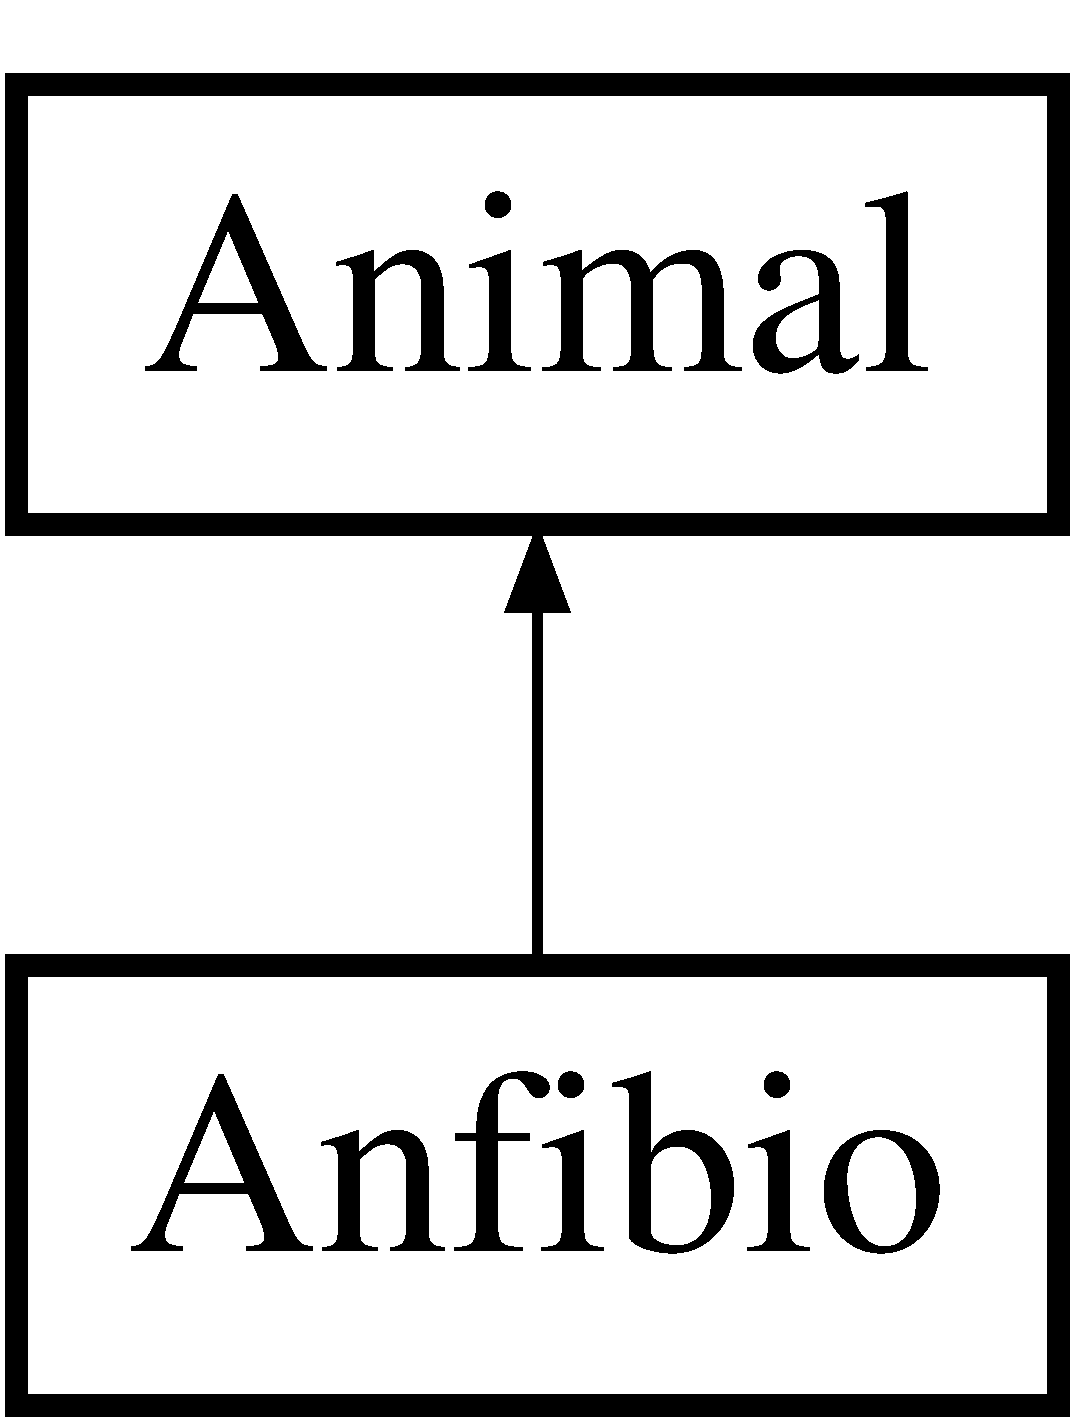
\includegraphics[height=2.000000cm]{classAnfibio}
\end{center}
\end{figure}
\subsection*{Public Member Functions}
\begin{DoxyCompactItemize}
\item 
\mbox{\Hypertarget{classAnfibio_aebbf81fc5e9f86b2e42bcdfe52ab7514}\label{classAnfibio_aebbf81fc5e9f86b2e42bcdfe52ab7514}} 
{\bfseries Anfibio} (std\+::string \+\_\+id, std\+::string \+\_\+classe, std\+::string \+\_\+nome\+\_\+especie, std\+::string \+\_\+nome\+\_\+cientifico, char \+\_\+sexo, float \+\_\+tamanho, std\+::string \+\_\+dieta, \hyperlink{classVeterinario}{Veterinario} \&\+\_\+veterinario, \hyperlink{classTratador}{Tratador} \&\+\_\+tratador, std\+::string \+\_\+nome\+\_\+de\+\_\+batismo, int \+\_\+mudas\+\_\+ja\+\_\+realizadas, std\+::string \+\_\+ultima\+\_\+muda)
\item 
\mbox{\Hypertarget{classAnfibio_a3c18155735838879de283120c1ccf4a4}\label{classAnfibio_a3c18155735838879de283120c1ccf4a4}} 
void {\bfseries set\+Ultima\+Muda} (std\+::string \+\_\+ultima\+\_\+muda)
\item 
\mbox{\Hypertarget{classAnfibio_a7dbb38f199ce548803f9f688a4041d5e}\label{classAnfibio_a7dbb38f199ce548803f9f688a4041d5e}} 
int {\bfseries get\+Mudas\+Ja\+Realizadas} ()
\item 
\mbox{\Hypertarget{classAnfibio_a8ae043bc3b2cd178817eb4d97a6da5aa}\label{classAnfibio_a8ae043bc3b2cd178817eb4d97a6da5aa}} 
std\+::string {\bfseries get\+Ultima\+Muda} ()
\item 
\mbox{\Hypertarget{classAnfibio_a0e38cc3c4c3cad0233d118d46775a1b6}\label{classAnfibio_a0e38cc3c4c3cad0233d118d46775a1b6}} 
std\+::ostream \& {\bfseries print} (std\+::ostream \&o)
\end{DoxyCompactItemize}
\subsection*{Protected Attributes}
\begin{DoxyCompactItemize}
\item 
\mbox{\Hypertarget{classAnfibio_a5d87808f8ed0adbf601c582c7e8093d1}\label{classAnfibio_a5d87808f8ed0adbf601c582c7e8093d1}} 
int {\bfseries mudas\+\_\+ja\+\_\+realizadas}
\item 
\mbox{\Hypertarget{classAnfibio_ae859b67a63a815463e07f776d43de4ff}\label{classAnfibio_ae859b67a63a815463e07f776d43de4ff}} 
std\+::string {\bfseries ultima\+\_\+muda}
\end{DoxyCompactItemize}


The documentation for this class was generated from the following files\+:\begin{DoxyCompactItemize}
\item 
/home/xsolowingx/\+L\+P1/\+Programas/\+Projeto3/include/\hyperlink{anfibio_8h}{anfibio.\+h}\item 
/home/xsolowingx/\+L\+P1/\+Programas/\+Projeto3/src/\hyperlink{anfibio_8cpp}{anfibio.\+cpp}\end{DoxyCompactItemize}

\hypertarget{classAnimal}{}\section{Animal Class Reference}
\label{classAnimal}\index{Animal@{Animal}}
Inheritance diagram for Animal\+:\begin{figure}[H]
\begin{center}
\leavevmode
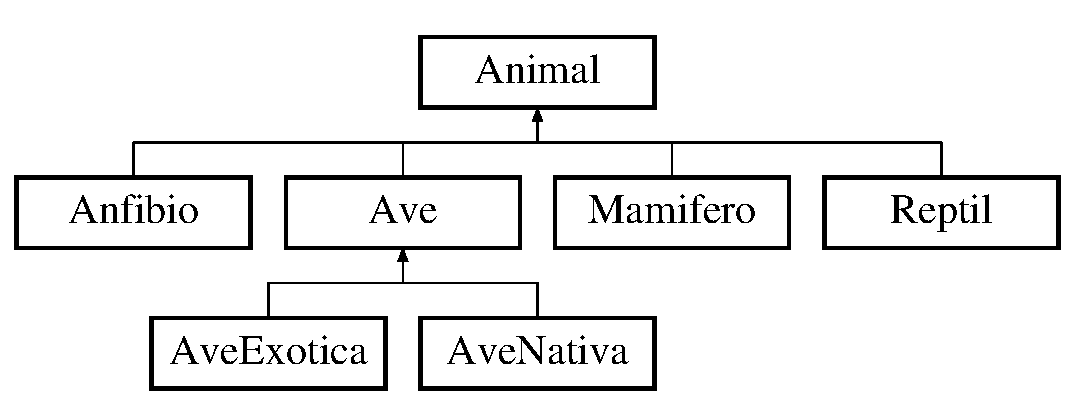
\includegraphics[height=3.000000cm]{classAnimal}
\end{center}
\end{figure}
\subsection*{Public Member Functions}
\begin{DoxyCompactItemize}
\item 
\mbox{\Hypertarget{classAnimal_a99fe9393f253449052651d550d124a5f}\label{classAnimal_a99fe9393f253449052651d550d124a5f}} 
{\bfseries Animal} (std\+::string \+\_\+id, std\+::string \+\_\+classe, std\+::string \+\_\+nome\+\_\+especie, std\+::string \+\_\+nome\+\_\+cientifico, char \+\_\+sexo, float \+\_\+tamanho, std\+::string \+\_\+dieta, \hyperlink{classVeterinario}{Veterinario} \&\+\_\+veterinario, \hyperlink{classTratador}{Tratador} \&\+\_\+tratador, std\+::string \+\_\+nome\+\_\+de\+\_\+batismo)
\item 
\mbox{\Hypertarget{classAnimal_ab8240e383d61d986083c21947d232b05}\label{classAnimal_ab8240e383d61d986083c21947d232b05}} 
void {\bfseries set\+Veterinario} (\hyperlink{classVeterinario}{Veterinario} \&\+\_\+veterinario)
\item 
\mbox{\Hypertarget{classAnimal_ab6ab444f36053a042ff48beba0827138}\label{classAnimal_ab6ab444f36053a042ff48beba0827138}} 
void {\bfseries set\+Tratador} (\hyperlink{classTratador}{Tratador} \&\+\_\+tratador)
\item 
\mbox{\Hypertarget{classAnimal_a7c90e853bf9f77be8d1cf7e2583acdd6}\label{classAnimal_a7c90e853bf9f77be8d1cf7e2583acdd6}} 
void {\bfseries set\+Tamanho} (float \+\_\+tamanho)
\item 
\mbox{\Hypertarget{classAnimal_ae6fb5bbe6940fd1e4ce43ff1a5dbffc1}\label{classAnimal_ae6fb5bbe6940fd1e4ce43ff1a5dbffc1}} 
std\+::string {\bfseries get\+Veterinario} ()
\item 
\mbox{\Hypertarget{classAnimal_abe5e5ecbc9c3f7da286091637c6e69d2}\label{classAnimal_abe5e5ecbc9c3f7da286091637c6e69d2}} 
std\+::string {\bfseries get\+Tratador} ()
\item 
\mbox{\Hypertarget{classAnimal_a22e54ff48117237f9a201f5eca0eea81}\label{classAnimal_a22e54ff48117237f9a201f5eca0eea81}} 
std\+::string {\bfseries get\+Classe} ()
\item 
\mbox{\Hypertarget{classAnimal_aab90929d32083cd33cb22df862fbff82}\label{classAnimal_aab90929d32083cd33cb22df862fbff82}} 
virtual std\+::ostream \& {\bfseries print} (std\+::ostream \&o)=0
\end{DoxyCompactItemize}
\subsection*{Protected Attributes}
\begin{DoxyCompactItemize}
\item 
\mbox{\Hypertarget{classAnimal_a680dc3aa9dfaa9a9fa3abd564ec91a9f}\label{classAnimal_a680dc3aa9dfaa9a9fa3abd564ec91a9f}} 
std\+::string {\bfseries id}
\item 
\mbox{\Hypertarget{classAnimal_aa5a6a3e322de28da865a7e2a91b9416d}\label{classAnimal_aa5a6a3e322de28da865a7e2a91b9416d}} 
std\+::string {\bfseries classe}
\item 
\mbox{\Hypertarget{classAnimal_abc4601e5206852c0bb757e73e461eda2}\label{classAnimal_abc4601e5206852c0bb757e73e461eda2}} 
std\+::string {\bfseries nome\+\_\+especie}
\item 
\mbox{\Hypertarget{classAnimal_a5a5861cf1a9abf2c9e26342f07cf4de5}\label{classAnimal_a5a5861cf1a9abf2c9e26342f07cf4de5}} 
std\+::string {\bfseries nome\+\_\+cientifico}
\item 
\mbox{\Hypertarget{classAnimal_a1fed4a4c287d4a9507e718692eb2837a}\label{classAnimal_a1fed4a4c287d4a9507e718692eb2837a}} 
char {\bfseries sexo}
\item 
\mbox{\Hypertarget{classAnimal_af164439fb6b2f4c470f451a8e7cbfd1e}\label{classAnimal_af164439fb6b2f4c470f451a8e7cbfd1e}} 
float {\bfseries tamanho}
\item 
\mbox{\Hypertarget{classAnimal_a253b474ae6bc13d122d07ff22d6aabc5}\label{classAnimal_a253b474ae6bc13d122d07ff22d6aabc5}} 
std\+::string {\bfseries dieta}
\item 
\mbox{\Hypertarget{classAnimal_a3618cd50da896cee0b62eec659d2c2bb}\label{classAnimal_a3618cd50da896cee0b62eec659d2c2bb}} 
\hyperlink{classVeterinario}{Veterinario} {\bfseries veterinario}
\item 
\mbox{\Hypertarget{classAnimal_a9a864369990c6743895032c6c8f2bdbc}\label{classAnimal_a9a864369990c6743895032c6c8f2bdbc}} 
\hyperlink{classTratador}{Tratador} {\bfseries tratador}
\item 
\mbox{\Hypertarget{classAnimal_a49467456bdef4eee33c271fa702c5f02}\label{classAnimal_a49467456bdef4eee33c271fa702c5f02}} 
std\+::string {\bfseries nome\+\_\+de\+\_\+batismo}
\end{DoxyCompactItemize}
\subsection*{Friends}
\begin{DoxyCompactItemize}
\item 
\mbox{\Hypertarget{classAnimal_a60e87f6bdfb739354180c27be7186c0a}\label{classAnimal_a60e87f6bdfb739354180c27be7186c0a}} 
std\+::ostream \& {\bfseries operator$<$$<$} (std\+::ostream \&o, \hyperlink{classAnimal}{Animal} \&a)
\end{DoxyCompactItemize}


The documentation for this class was generated from the following files\+:\begin{DoxyCompactItemize}
\item 
/home/xsolowingx/\+L\+P1/\+Programas/\+Projeto3/include/\hyperlink{animal_8h}{animal.\+h}\item 
/home/xsolowingx/\+L\+P1/\+Programas/\+Projeto3/src/\hyperlink{animal_8cpp}{animal.\+cpp}\end{DoxyCompactItemize}

\hypertarget{classAnimalSilvestre}{}\section{Animal\+Silvestre Class Reference}
\label{classAnimalSilvestre}\index{Animal\+Silvestre@{Animal\+Silvestre}}
Inheritance diagram for Animal\+Silvestre\+:\begin{figure}[H]
\begin{center}
\leavevmode
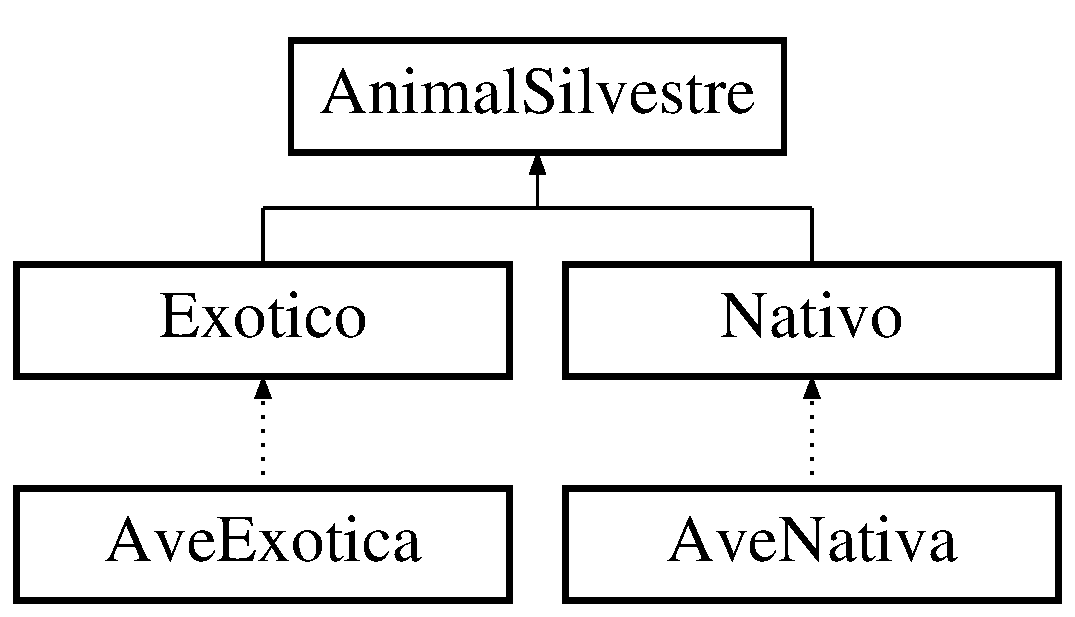
\includegraphics[height=3.000000cm]{classAnimalSilvestre}
\end{center}
\end{figure}
\subsection*{Public Member Functions}
\begin{DoxyCompactItemize}
\item 
\mbox{\Hypertarget{classAnimalSilvestre_ab2d89bd466c5dfa210fd8777c8f67f2c}\label{classAnimalSilvestre_ab2d89bd466c5dfa210fd8777c8f67f2c}} 
{\bfseries Animal\+Silvestre} (std\+::string \+\_\+permissao\+\_\+ibama)
\item 
\mbox{\Hypertarget{classAnimalSilvestre_a9cf5ef01a13af94712ec39916edd09ea}\label{classAnimalSilvestre_a9cf5ef01a13af94712ec39916edd09ea}} 
void {\bfseries set\+Permissao} (std\+::string \+\_\+permission)
\item 
\mbox{\Hypertarget{classAnimalSilvestre_a99b340ebe3717d03b31455c565afd5ad}\label{classAnimalSilvestre_a99b340ebe3717d03b31455c565afd5ad}} 
virtual std\+::string {\bfseries get\+Permissao} () const =0
\end{DoxyCompactItemize}
\subsection*{Protected Attributes}
\begin{DoxyCompactItemize}
\item 
\mbox{\Hypertarget{classAnimalSilvestre_afe5c61c862f252fadbb2c9779ed67592}\label{classAnimalSilvestre_afe5c61c862f252fadbb2c9779ed67592}} 
std\+::string {\bfseries permissao\+\_\+ibama}
\end{DoxyCompactItemize}


The documentation for this class was generated from the following files\+:\begin{DoxyCompactItemize}
\item 
/home/xsolowingx/\+L\+P1/\+Programas/\+Projeto3/include/\hyperlink{animalSilvestre_8h}{animal\+Silvestre.\+h}\item 
/home/xsolowingx/\+L\+P1/\+Programas/\+Projeto3/src/\hyperlink{animalSilvestre_8cpp}{animal\+Silvestre.\+cpp}\end{DoxyCompactItemize}

\hypertarget{classAve}{}\section{Ave Class Reference}
\label{classAve}\index{Ave@{Ave}}
Inheritance diagram for Ave\+:\begin{figure}[H]
\begin{center}
\leavevmode
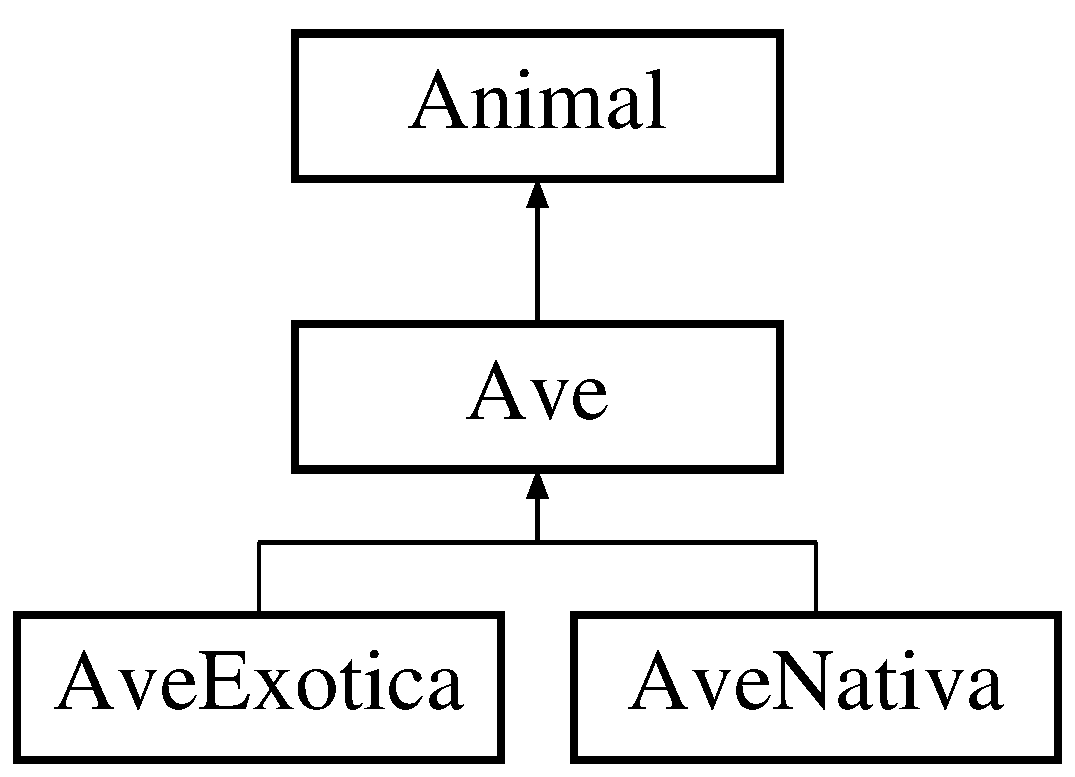
\includegraphics[height=3.000000cm]{classAve}
\end{center}
\end{figure}
\subsection*{Public Member Functions}
\begin{DoxyCompactItemize}
\item 
\mbox{\Hypertarget{classAve_a7c147f6153c466ae6a744ffd1c3aa380}\label{classAve_a7c147f6153c466ae6a744ffd1c3aa380}} 
{\bfseries Ave} (std\+::string \+\_\+id, std\+::string \+\_\+classe, std\+::string \+\_\+nome\+\_\+especie, std\+::string \+\_\+nome\+\_\+cientifico, char \+\_\+sexo, float \+\_\+tamanho, std\+::string \+\_\+dieta, \hyperlink{classVeterinario}{Veterinario} \&\+\_\+veterinario, \hyperlink{classTratador}{Tratador} \&\+\_\+tratador, std\+::string \+\_\+nome\+\_\+de\+\_\+batismo, int \+\_\+tamanho\+\_\+do\+\_\+bico, int \+\_\+envergadura)
\item 
\mbox{\Hypertarget{classAve_a5fb81fec98f756fdaae84e0ed31df7fa}\label{classAve_a5fb81fec98f756fdaae84e0ed31df7fa}} 
void {\bfseries set\+Tamanho\+Do\+Bico} (int \+\_\+tb)
\item 
\mbox{\Hypertarget{classAve_a1384b352a4844d546258124d6f353532}\label{classAve_a1384b352a4844d546258124d6f353532}} 
void {\bfseries set\+Envergadura} (int \+\_\+enve)
\item 
\mbox{\Hypertarget{classAve_ac0c89141e2670b7f7f827327ba97aafe}\label{classAve_ac0c89141e2670b7f7f827327ba97aafe}} 
int {\bfseries get\+Tamanho\+Do\+Bico} ()
\item 
\mbox{\Hypertarget{classAve_acf18daa406f41e12d4cca32c7c451371}\label{classAve_acf18daa406f41e12d4cca32c7c451371}} 
int {\bfseries get\+Envergadura} ()
\item 
\mbox{\Hypertarget{classAve_a9cb34958345b998e68804d0bcc44a6d0}\label{classAve_a9cb34958345b998e68804d0bcc44a6d0}} 
std\+::ostream \& {\bfseries print} (std\+::ostream \&o)
\end{DoxyCompactItemize}
\subsection*{Protected Attributes}
\begin{DoxyCompactItemize}
\item 
\mbox{\Hypertarget{classAve_ad31143f96b75f003b87d3823a7af1ae8}\label{classAve_ad31143f96b75f003b87d3823a7af1ae8}} 
int {\bfseries tamanho\+\_\+do\+\_\+bico}
\item 
\mbox{\Hypertarget{classAve_acd66c7ac8887d8eecbe3e15a8508b25d}\label{classAve_acd66c7ac8887d8eecbe3e15a8508b25d}} 
int {\bfseries envergadura}
\end{DoxyCompactItemize}


The documentation for this class was generated from the following files\+:\begin{DoxyCompactItemize}
\item 
/home/xsolowingx/\+L\+P1/\+Programas/\+Projeto3/include/\hyperlink{ave_8h}{ave.\+h}\item 
/home/xsolowingx/\+L\+P1/\+Programas/\+Projeto3/src/\hyperlink{ave_8cpp}{ave.\+cpp}\end{DoxyCompactItemize}

\hypertarget{classAveExotica}{}\section{Ave\+Exotica Class Reference}
\label{classAveExotica}\index{Ave\+Exotica@{Ave\+Exotica}}
Inheritance diagram for Ave\+Exotica\+:\begin{figure}[H]
\begin{center}
\leavevmode
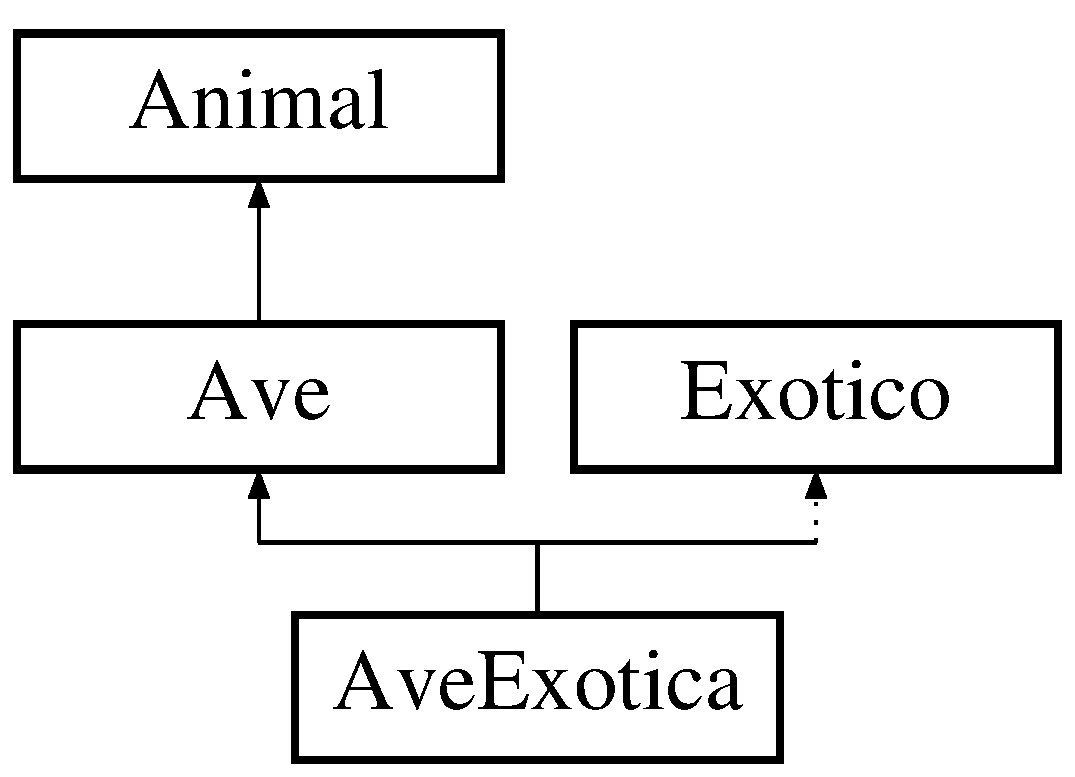
\includegraphics[height=3.000000cm]{classAveExotica}
\end{center}
\end{figure}
\subsection*{Public Member Functions}
\begin{DoxyCompactItemize}
\item 
\mbox{\Hypertarget{classAveExotica_aecd13c8d769ad45e46fb3393a7832997}\label{classAveExotica_aecd13c8d769ad45e46fb3393a7832997}} 
{\bfseries Ave\+Exotica} (std\+::string \+\_\+id, std\+::string \+\_\+classe, std\+::string \+\_\+nome\+\_\+especie, std\+::string \+\_\+nome\+\_\+cientifico, char \+\_\+sexo, float \+\_\+tamanho, std\+::string \+\_\+dieta, \hyperlink{classVeterinario}{Veterinario} \&\+\_\+veterinario, \hyperlink{classTratador}{Tratador} \&\+\_\+tratador, std\+::string \+\_\+nome\+\_\+de\+\_\+batismo, int \+\_\+tamanho\+\_\+do\+\_\+bico, int \+\_\+envergadura, std\+::string \+\_\+permissao\+\_\+ibama, std\+::string \+\_\+pais\+\_\+de\+\_\+origem)
\item 
\mbox{\Hypertarget{classAveExotica_adccbd74661ee6f633e79229ae6e0bf5b}\label{classAveExotica_adccbd74661ee6f633e79229ae6e0bf5b}} 
std\+::string {\bfseries get\+Pais\+De\+Origem} () const
\item 
\mbox{\Hypertarget{classAveExotica_a8c6fbe0ed75a48003087db98525664d1}\label{classAveExotica_a8c6fbe0ed75a48003087db98525664d1}} 
std\+::string {\bfseries get\+Permissao} () const
\end{DoxyCompactItemize}
\subsection*{Additional Inherited Members}


The documentation for this class was generated from the following files\+:\begin{DoxyCompactItemize}
\item 
/home/xsolowingx/\+L\+P1/\+Programas/\+Projeto3/include/\hyperlink{aveExotica_8h}{ave\+Exotica.\+h}\item 
/home/xsolowingx/\+L\+P1/\+Programas/\+Projeto3/src/\hyperlink{aveExotica_8cpp}{ave\+Exotica.\+cpp}\end{DoxyCompactItemize}

\hypertarget{classAveNativa}{}\section{Ave\+Nativa Class Reference}
\label{classAveNativa}\index{Ave\+Nativa@{Ave\+Nativa}}
Inheritance diagram for Ave\+Nativa\+:\begin{figure}[H]
\begin{center}
\leavevmode
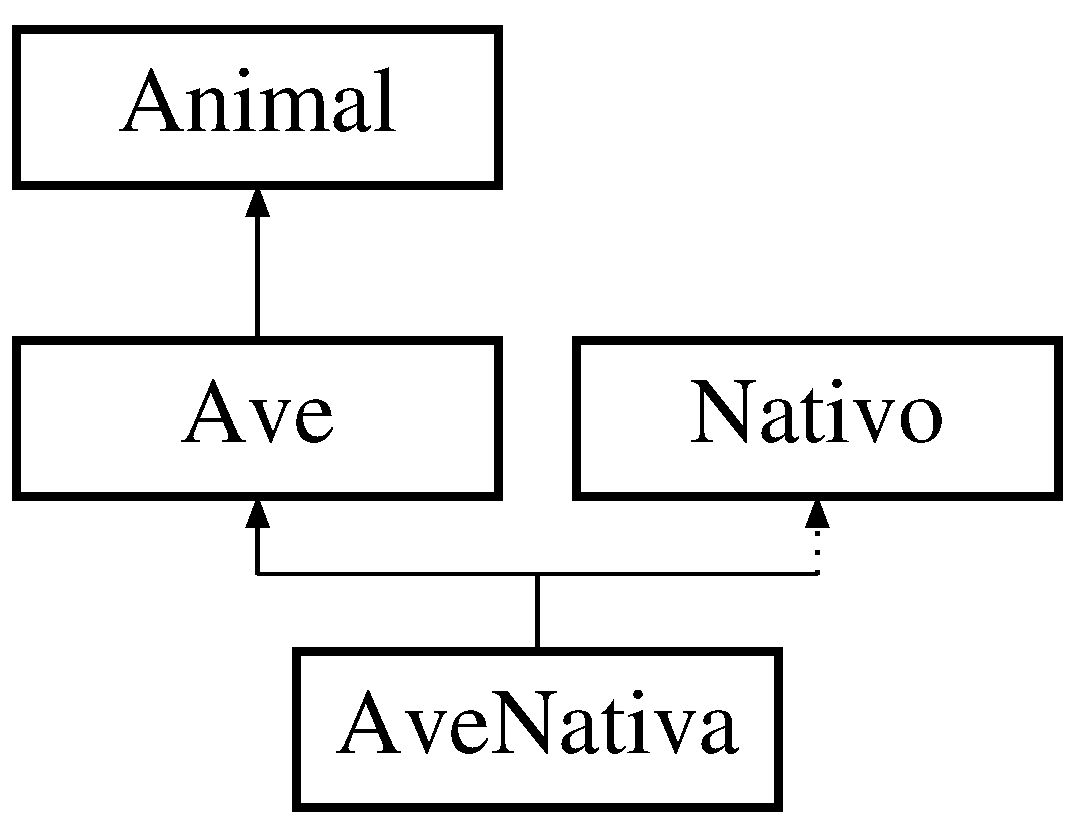
\includegraphics[height=3.000000cm]{classAveNativa}
\end{center}
\end{figure}
\subsection*{Public Member Functions}
\begin{DoxyCompactItemize}
\item 
\mbox{\Hypertarget{classAveNativa_abbb03ed031a100c5f8268cdfb644d0f7}\label{classAveNativa_abbb03ed031a100c5f8268cdfb644d0f7}} 
{\bfseries Ave\+Nativa} (std\+::string \+\_\+id, std\+::string \+\_\+classe, std\+::string \+\_\+nome\+\_\+especie, std\+::string \+\_\+nome\+\_\+cientifico, char \+\_\+sexo, float \+\_\+tamanho, std\+::string \+\_\+dieta, \hyperlink{classVeterinario}{Veterinario} \&\+\_\+veterinario, \hyperlink{classTratador}{Tratador} \&\+\_\+tratador, std\+::string \+\_\+nome\+\_\+de\+\_\+batismo, int \+\_\+tamanho\+\_\+do\+\_\+bico, int \+\_\+envergadura, std\+::string \+\_\+permissao\+\_\+ibama, std\+::string \+\_\+estado\+\_\+de\+\_\+origem, std\+::string \+\_\+autorizacao)
\item 
\mbox{\Hypertarget{classAveNativa_a5946d2b5196fc4a99d33ae2be3deb40f}\label{classAveNativa_a5946d2b5196fc4a99d33ae2be3deb40f}} 
std\+::string {\bfseries get\+Permissao} () const
\item 
\mbox{\Hypertarget{classAveNativa_a83e72a38bc4c079a66617ffe2da38bd5}\label{classAveNativa_a83e72a38bc4c079a66617ffe2da38bd5}} 
std\+::string {\bfseries get\+Estado\+De\+Origem} () const
\item 
\mbox{\Hypertarget{classAveNativa_a2e87ed537e1de4041632e67e93d7f875}\label{classAveNativa_a2e87ed537e1de4041632e67e93d7f875}} 
std\+::string {\bfseries get\+Autorizacao} () const
\end{DoxyCompactItemize}
\subsection*{Additional Inherited Members}


The documentation for this class was generated from the following files\+:\begin{DoxyCompactItemize}
\item 
/home/xsolowingx/\+L\+P1/\+Programas/\+Projeto3/include/\hyperlink{aveNativa_8h}{ave\+Nativa.\+h}\item 
/home/xsolowingx/\+L\+P1/\+Programas/\+Projeto3/src/\hyperlink{aveNativa_8cpp}{ave\+Nativa.\+cpp}\end{DoxyCompactItemize}

\hypertarget{classErroAoAbrirArquivo}{}\section{Erro\+Ao\+Abrir\+Arquivo Class Reference}
\label{classErroAoAbrirArquivo}\index{Erro\+Ao\+Abrir\+Arquivo@{Erro\+Ao\+Abrir\+Arquivo}}
Inheritance diagram for Erro\+Ao\+Abrir\+Arquivo\+:\begin{figure}[H]
\begin{center}
\leavevmode
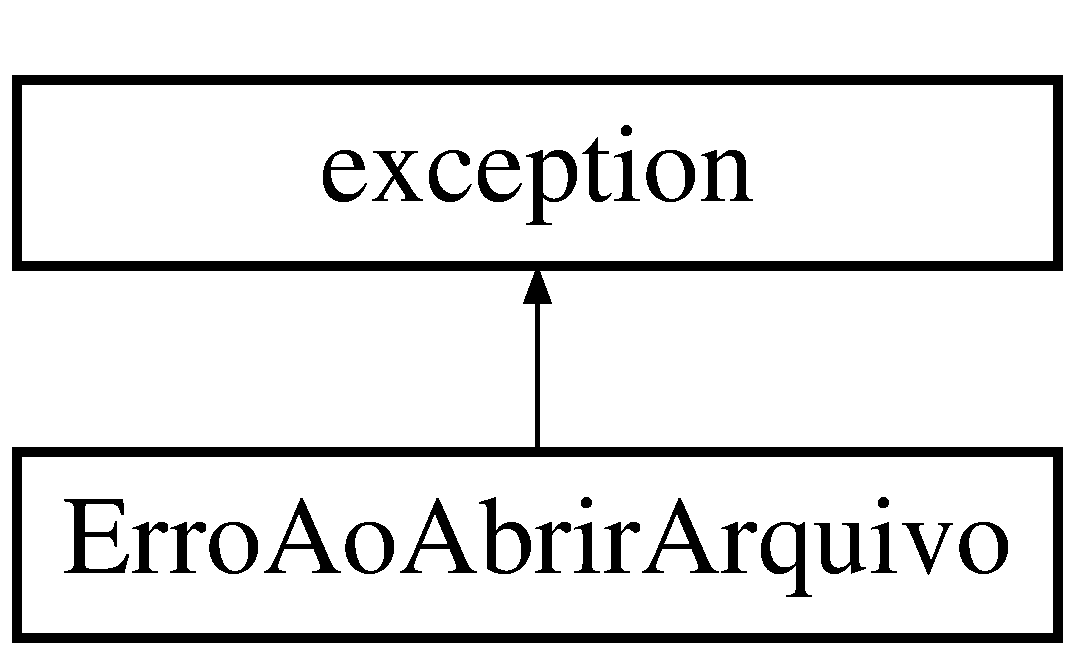
\includegraphics[height=2.000000cm]{classErroAoAbrirArquivo}
\end{center}
\end{figure}
\subsection*{Public Member Functions}
\begin{DoxyCompactItemize}
\item 
\mbox{\Hypertarget{classErroAoAbrirArquivo_a82ff15bef3608ab854b3621dedd25be8}\label{classErroAoAbrirArquivo_a82ff15bef3608ab854b3621dedd25be8}} 
const char $\ast$ {\bfseries what} ()
\end{DoxyCompactItemize}


The documentation for this class was generated from the following files\+:\begin{DoxyCompactItemize}
\item 
/home/xsolowingx/\+L\+P1/\+Programas/\+Projeto3/include/\hyperlink{excecoes_8h}{excecoes.\+h}\item 
/home/xsolowingx/\+L\+P1/\+Programas/\+Projeto3/src/\hyperlink{excecoes_8cpp}{excecoes.\+cpp}\end{DoxyCompactItemize}

\hypertarget{classErroAoTentarLerDados}{}\section{Erro\+Ao\+Tentar\+Ler\+Dados Class Reference}
\label{classErroAoTentarLerDados}\index{Erro\+Ao\+Tentar\+Ler\+Dados@{Erro\+Ao\+Tentar\+Ler\+Dados}}
Inheritance diagram for Erro\+Ao\+Tentar\+Ler\+Dados\+:\begin{figure}[H]
\begin{center}
\leavevmode
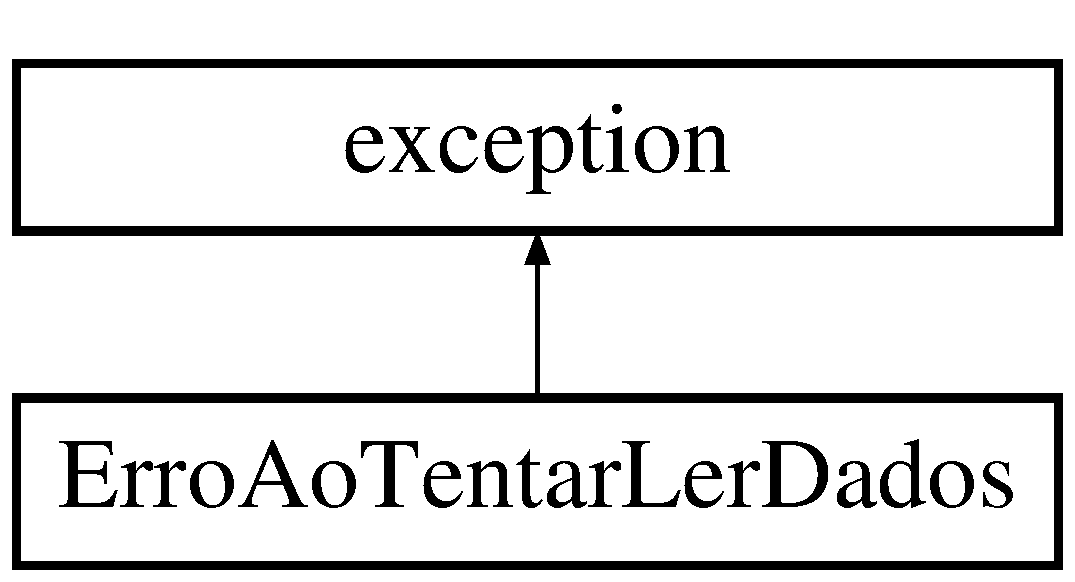
\includegraphics[height=2.000000cm]{classErroAoTentarLerDados}
\end{center}
\end{figure}
\subsection*{Public Member Functions}
\begin{DoxyCompactItemize}
\item 
\mbox{\Hypertarget{classErroAoTentarLerDados_a0a0b41c84affe6dbdc4b7f06bb542099}\label{classErroAoTentarLerDados_a0a0b41c84affe6dbdc4b7f06bb542099}} 
const char $\ast$ {\bfseries what} ()
\end{DoxyCompactItemize}


The documentation for this class was generated from the following files\+:\begin{DoxyCompactItemize}
\item 
/home/xsolowingx/\+L\+P1/\+Programas/\+Projeto3/include/\hyperlink{excecoes_8h}{excecoes.\+h}\item 
/home/xsolowingx/\+L\+P1/\+Programas/\+Projeto3/src/\hyperlink{excecoes_8cpp}{excecoes.\+cpp}\end{DoxyCompactItemize}

\hypertarget{classExotico}{}\section{Exotico Class Reference}
\label{classExotico}\index{Exotico@{Exotico}}
Inheritance diagram for Exotico\+:\begin{figure}[H]
\begin{center}
\leavevmode
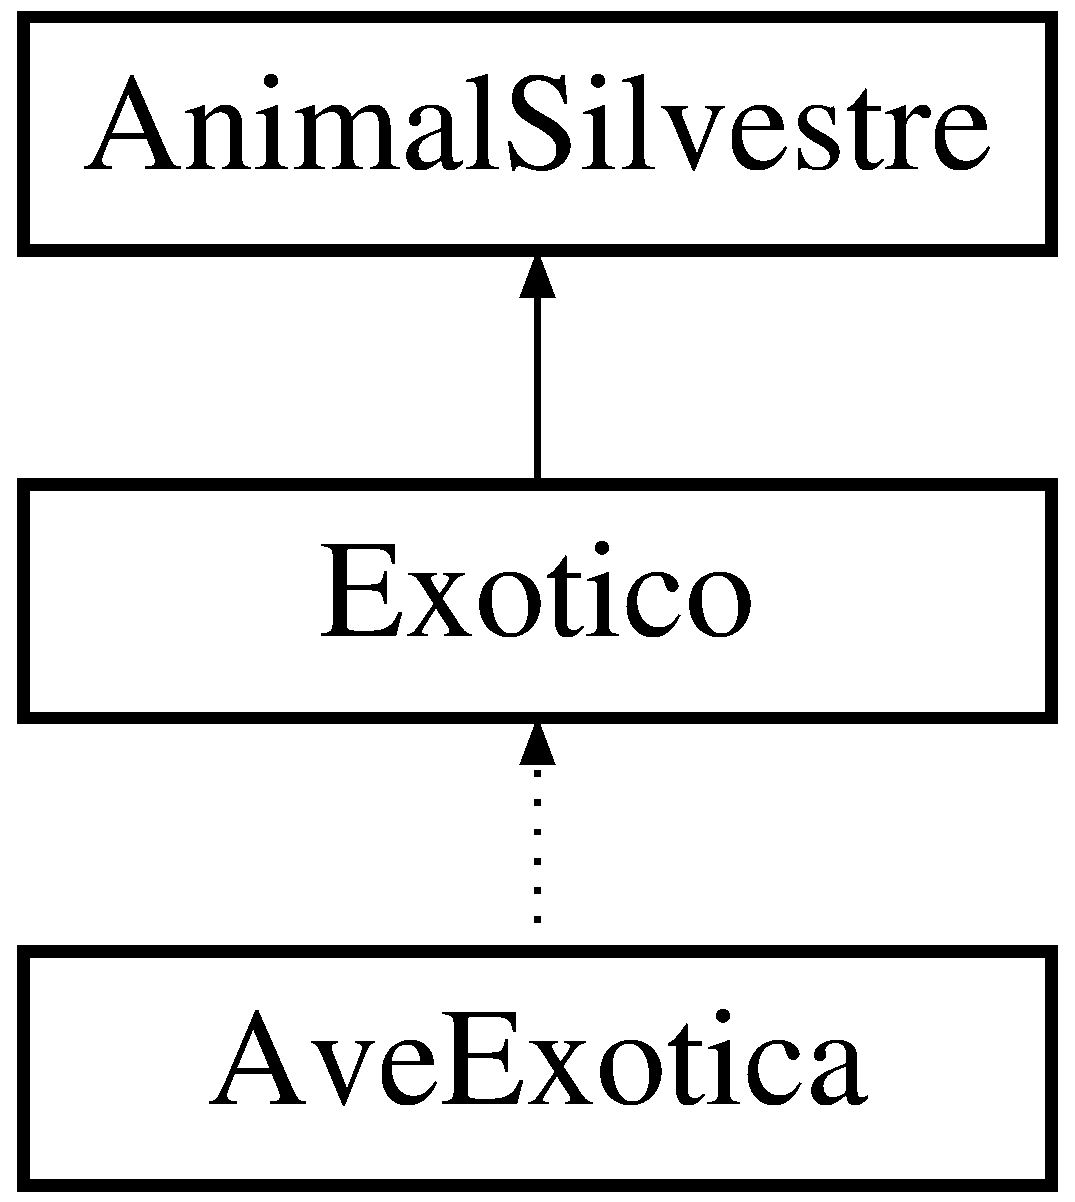
\includegraphics[height=3.000000cm]{classExotico}
\end{center}
\end{figure}
\subsection*{Public Member Functions}
\begin{DoxyCompactItemize}
\item 
\mbox{\Hypertarget{classExotico_a810d1ec34106e9c2ec6b725af40bcdbf}\label{classExotico_a810d1ec34106e9c2ec6b725af40bcdbf}} 
{\bfseries Exotico} (std\+::string \+\_\+permissao\+\_\+ibama, std\+::string \+\_\+pais\+\_\+de\+\_\+origem)
\item 
\mbox{\Hypertarget{classExotico_ae0ee8fb011ca22acd674ac8fcf8917dd}\label{classExotico_ae0ee8fb011ca22acd674ac8fcf8917dd}} 
virtual std\+::string {\bfseries get\+Pais\+De\+Origem} () const =0
\item 
\mbox{\Hypertarget{classExotico_a3fa36660107b1af74272a7ae0f297239}\label{classExotico_a3fa36660107b1af74272a7ae0f297239}} 
virtual std\+::string {\bfseries get\+Permissao} () const =0
\end{DoxyCompactItemize}
\subsection*{Protected Attributes}
\begin{DoxyCompactItemize}
\item 
\mbox{\Hypertarget{classExotico_ae1a8fad5cd213e89fff278c4a928f169}\label{classExotico_ae1a8fad5cd213e89fff278c4a928f169}} 
std\+::string {\bfseries pais\+\_\+de\+\_\+origem}
\end{DoxyCompactItemize}


The documentation for this class was generated from the following files\+:\begin{DoxyCompactItemize}
\item 
/home/xsolowingx/\+L\+P1/\+Programas/\+Projeto3/include/\hyperlink{exotico_8h}{exotico.\+h}\item 
/home/xsolowingx/\+L\+P1/\+Programas/\+Projeto3/src/\hyperlink{exotico_8cpp}{exotico.\+cpp}\end{DoxyCompactItemize}

\hypertarget{classFuncionario}{}\section{Funcionario Class Reference}
\label{classFuncionario}\index{Funcionario@{Funcionario}}
Inheritance diagram for Funcionario\+:\begin{figure}[H]
\begin{center}
\leavevmode
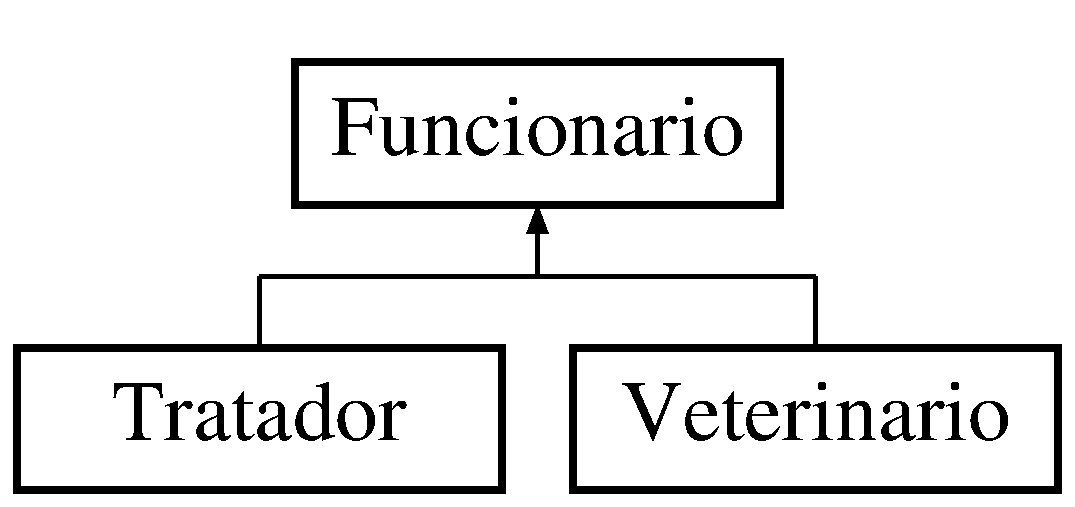
\includegraphics[height=2.000000cm]{classFuncionario}
\end{center}
\end{figure}
\subsection*{Public Member Functions}
\begin{DoxyCompactItemize}
\item 
\mbox{\Hypertarget{classFuncionario_a600d73bb607ec21e94050eb09967dc3a}\label{classFuncionario_a600d73bb607ec21e94050eb09967dc3a}} 
{\bfseries Funcionario} (std\+::string \+\_\+id, std\+::string \+\_\+nome, std\+::string \+\_\+cpf, std\+::string \+\_\+idade, std\+::string \+\_\+tipo\+\_\+sanguineo, std\+::string \+\_\+fator\+RH, std\+::string \+\_\+especialidade, std\+::string \+\_\+funcao)
\item 
\mbox{\Hypertarget{classFuncionario_a851eb221b3725471ccffe576fc268780}\label{classFuncionario_a851eb221b3725471ccffe576fc268780}} 
void {\bfseries set\+ID} (std\+::string \+\_\+id)
\item 
\mbox{\Hypertarget{classFuncionario_abbea04f5d58470005b8eef8702aefe7a}\label{classFuncionario_abbea04f5d58470005b8eef8702aefe7a}} 
void {\bfseries set\+Nome} (std\+::string \+\_\+nome)
\item 
\mbox{\Hypertarget{classFuncionario_a1de87beb63644d6eaf01a760329556b2}\label{classFuncionario_a1de87beb63644d6eaf01a760329556b2}} 
void {\bfseries set\+C\+PF} (std\+::string \+\_\+cpf)
\item 
\mbox{\Hypertarget{classFuncionario_a7536e578810b4816b37a329d2323b8a0}\label{classFuncionario_a7536e578810b4816b37a329d2323b8a0}} 
void {\bfseries set\+Idade} (std\+::string \+\_\+idade)
\item 
\mbox{\Hypertarget{classFuncionario_a67503361a14954680bc6a20024516331}\label{classFuncionario_a67503361a14954680bc6a20024516331}} 
void {\bfseries set\+Tipo\+Sanguineo} (std\+::string \+\_\+tipo\+\_\+sanguineo)
\item 
\mbox{\Hypertarget{classFuncionario_a6b565d63121fe52013a8368c8554188a}\label{classFuncionario_a6b565d63121fe52013a8368c8554188a}} 
void {\bfseries set\+Fator\+RH} (std\+::string \+\_\+fator\+RH)
\item 
\mbox{\Hypertarget{classFuncionario_a33d68dffd2c432a04c3f3e1c6b3d969b}\label{classFuncionario_a33d68dffd2c432a04c3f3e1c6b3d969b}} 
void {\bfseries set\+Especialidade} (std\+::string \+\_\+especialidade)
\item 
\mbox{\Hypertarget{classFuncionario_a1f2c33c1db147ceb8d1b8c7e0694e168}\label{classFuncionario_a1f2c33c1db147ceb8d1b8c7e0694e168}} 
std\+::string {\bfseries get\+ID} ()
\item 
\mbox{\Hypertarget{classFuncionario_a35376709ae5c7357e79ca612a74e7f15}\label{classFuncionario_a35376709ae5c7357e79ca612a74e7f15}} 
std\+::string {\bfseries get\+Nome} ()
\item 
\mbox{\Hypertarget{classFuncionario_a15ca65608f1e7345ca5f99e79cdfa33b}\label{classFuncionario_a15ca65608f1e7345ca5f99e79cdfa33b}} 
std\+::string {\bfseries get\+C\+PF} ()
\item 
\mbox{\Hypertarget{classFuncionario_ac13a8bc1dd2425b3e316f0432e093a66}\label{classFuncionario_ac13a8bc1dd2425b3e316f0432e093a66}} 
std\+::string {\bfseries get\+Idade} ()
\item 
\mbox{\Hypertarget{classFuncionario_a871dfd5403d3d3c026c35b62ee2bb6a9}\label{classFuncionario_a871dfd5403d3d3c026c35b62ee2bb6a9}} 
std\+::string {\bfseries get\+Tipo\+Sanguineo} ()
\item 
\mbox{\Hypertarget{classFuncionario_adce524ef7422ef2bcc1b84c939f2d177}\label{classFuncionario_adce524ef7422ef2bcc1b84c939f2d177}} 
std\+::string {\bfseries get\+Fator\+RH} ()
\item 
\mbox{\Hypertarget{classFuncionario_a98b261893ff916049db28530d3ba1160}\label{classFuncionario_a98b261893ff916049db28530d3ba1160}} 
std\+::string {\bfseries get\+Especialidade} ()
\item 
\mbox{\Hypertarget{classFuncionario_a8e67899ba0fa720b95c0b292cfd6fe90}\label{classFuncionario_a8e67899ba0fa720b95c0b292cfd6fe90}} 
std\+::string {\bfseries get\+Funcao} ()
\item 
\mbox{\Hypertarget{classFuncionario_ae300f2d29776f6173d3267b314e31f24}\label{classFuncionario_ae300f2d29776f6173d3267b314e31f24}} 
virtual std\+::ostream \& {\bfseries print} (std\+::ostream \&o)=0
\item 
\mbox{\Hypertarget{classFuncionario_a615fd3db161ffe4425ec1bff06f1853f}\label{classFuncionario_a615fd3db161ffe4425ec1bff06f1853f}} 
virtual std\+::istream \& {\bfseries scan} (std\+::istream \&i)=0
\end{DoxyCompactItemize}
\subsection*{Protected Attributes}
\begin{DoxyCompactItemize}
\item 
\mbox{\Hypertarget{classFuncionario_a7c1e6557ef9b30185a2241a653a3da3e}\label{classFuncionario_a7c1e6557ef9b30185a2241a653a3da3e}} 
std\+::string {\bfseries id}
\item 
\mbox{\Hypertarget{classFuncionario_ac9e214af6fa91e21aa376a81e28f17ae}\label{classFuncionario_ac9e214af6fa91e21aa376a81e28f17ae}} 
std\+::string {\bfseries nome}
\item 
\mbox{\Hypertarget{classFuncionario_ab015f6593b7b62e7a9c2440dd334f97b}\label{classFuncionario_ab015f6593b7b62e7a9c2440dd334f97b}} 
std\+::string {\bfseries cpf}
\item 
\mbox{\Hypertarget{classFuncionario_abf6781eb509eb242b5067d6526ef9a01}\label{classFuncionario_abf6781eb509eb242b5067d6526ef9a01}} 
std\+::string {\bfseries idade}
\item 
\mbox{\Hypertarget{classFuncionario_a71fd2bf70bff1ed765bf7721ff22313e}\label{classFuncionario_a71fd2bf70bff1ed765bf7721ff22313e}} 
std\+::string {\bfseries tipo\+\_\+sanguineo}
\item 
\mbox{\Hypertarget{classFuncionario_a74e88a04cc9f8bcd1d88ebb1acc7f6f0}\label{classFuncionario_a74e88a04cc9f8bcd1d88ebb1acc7f6f0}} 
std\+::string {\bfseries fator\+RH}
\item 
\mbox{\Hypertarget{classFuncionario_a3cf1d47d414662e9ced6b0b4829d0316}\label{classFuncionario_a3cf1d47d414662e9ced6b0b4829d0316}} 
std\+::string {\bfseries especialidade}
\item 
\mbox{\Hypertarget{classFuncionario_ac82736fa17848d7f132e393a84a4c0c9}\label{classFuncionario_ac82736fa17848d7f132e393a84a4c0c9}} 
std\+::string {\bfseries funcao}
\end{DoxyCompactItemize}
\subsection*{Friends}
\begin{DoxyCompactItemize}
\item 
\mbox{\Hypertarget{classFuncionario_a2bb1f75049d15717556f551e25057e93}\label{classFuncionario_a2bb1f75049d15717556f551e25057e93}} 
std\+::istream \& {\bfseries operator$>$$>$} (std\+::istream \&i, \hyperlink{classFuncionario}{Funcionario} \&f)
\item 
\mbox{\Hypertarget{classFuncionario_abdee4494d45e2c0bb334c7ad2a9411c9}\label{classFuncionario_abdee4494d45e2c0bb334c7ad2a9411c9}} 
std\+::ostream \& {\bfseries operator$<$$<$} (std\+::ostream \&o, \hyperlink{classFuncionario}{Funcionario} \&f)
\end{DoxyCompactItemize}


The documentation for this class was generated from the following files\+:\begin{DoxyCompactItemize}
\item 
/home/xsolowingx/\+L\+P1/\+Programas/\+Projeto3/include/\hyperlink{funcionario_8h}{funcionario.\+h}\item 
/home/xsolowingx/\+L\+P1/\+Programas/\+Projeto3/src/\hyperlink{funcionario_8cpp}{funcionario.\+cpp}\end{DoxyCompactItemize}

\hypertarget{classMamifero}{}\section{Mamifero Class Reference}
\label{classMamifero}\index{Mamifero@{Mamifero}}
Inheritance diagram for Mamifero\+:\begin{figure}[H]
\begin{center}
\leavevmode
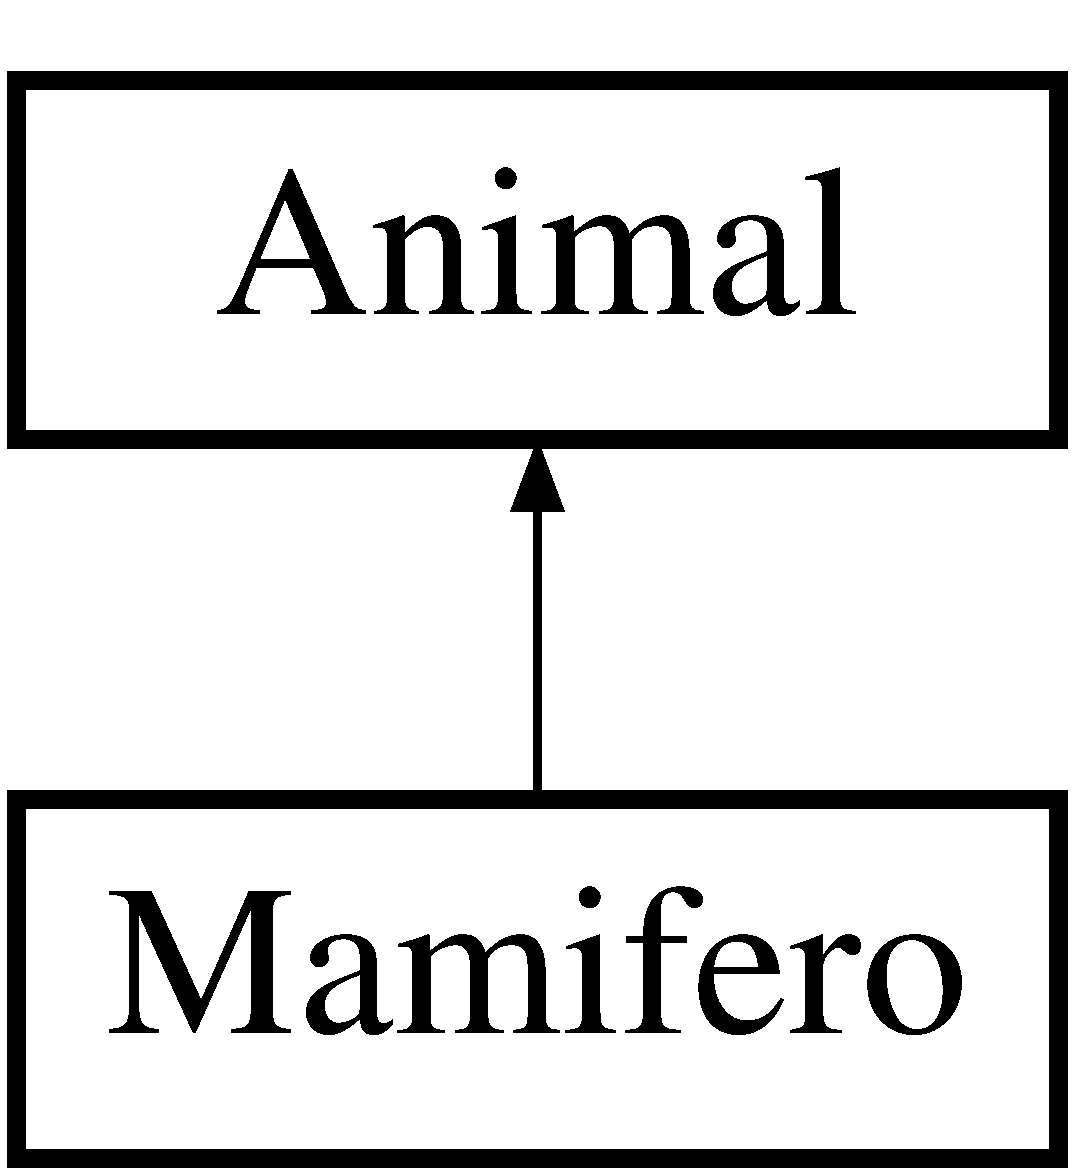
\includegraphics[height=2.000000cm]{classMamifero}
\end{center}
\end{figure}
\subsection*{Public Member Functions}
\begin{DoxyCompactItemize}
\item 
\mbox{\Hypertarget{classMamifero_a98c09018dcc79051f2a187d12e408a72}\label{classMamifero_a98c09018dcc79051f2a187d12e408a72}} 
{\bfseries Mamifero} (std\+::string \+\_\+id, std\+::string \+\_\+classe, std\+::string \+\_\+nome\+\_\+especie, std\+::string \+\_\+nome\+\_\+cientifico, char \+\_\+sexo, float \+\_\+tamanho, std\+::string \+\_\+dieta, \hyperlink{classVeterinario}{Veterinario} \&\+\_\+veterinario, \hyperlink{classTratador}{Tratador} \&\+\_\+tratador, std\+::string \+\_\+nome\+\_\+de\+\_\+batismo, std\+::string \+\_\+cor\+\_\+do\+\_\+pelo)
\item 
\mbox{\Hypertarget{classMamifero_ae7d1d9b7925e06c6fa34074a2654ff30}\label{classMamifero_ae7d1d9b7925e06c6fa34074a2654ff30}} 
void {\bfseries set\+Cor\+Do\+Pelo} (std\+::string \+\_\+cor)
\item 
\mbox{\Hypertarget{classMamifero_a7bf7c25d72549218df4472922ed365de}\label{classMamifero_a7bf7c25d72549218df4472922ed365de}} 
std\+::string {\bfseries get\+Cor\+Do\+Pelo} ()
\item 
\mbox{\Hypertarget{classMamifero_ae346f07cf380af1fc63f3fb4d88597d1}\label{classMamifero_ae346f07cf380af1fc63f3fb4d88597d1}} 
std\+::ostream \& {\bfseries print} (std\+::ostream \&o)
\end{DoxyCompactItemize}
\subsection*{Protected Attributes}
\begin{DoxyCompactItemize}
\item 
\mbox{\Hypertarget{classMamifero_a0fa2c0b3d670dbb657e6c5f112039327}\label{classMamifero_a0fa2c0b3d670dbb657e6c5f112039327}} 
std\+::string {\bfseries cor\+\_\+do\+\_\+pelo}
\end{DoxyCompactItemize}


The documentation for this class was generated from the following files\+:\begin{DoxyCompactItemize}
\item 
/home/xsolowingx/\+L\+P1/\+Programas/\+Projeto3/include/\hyperlink{mamifero_8h}{mamifero.\+h}\item 
/home/xsolowingx/\+L\+P1/\+Programas/\+Projeto3/src/\hyperlink{mamifero_8cpp}{mamifero.\+cpp}\end{DoxyCompactItemize}

\hypertarget{classNativo}{}\section{Nativo Class Reference}
\label{classNativo}\index{Nativo@{Nativo}}
Inheritance diagram for Nativo\+:\begin{figure}[H]
\begin{center}
\leavevmode
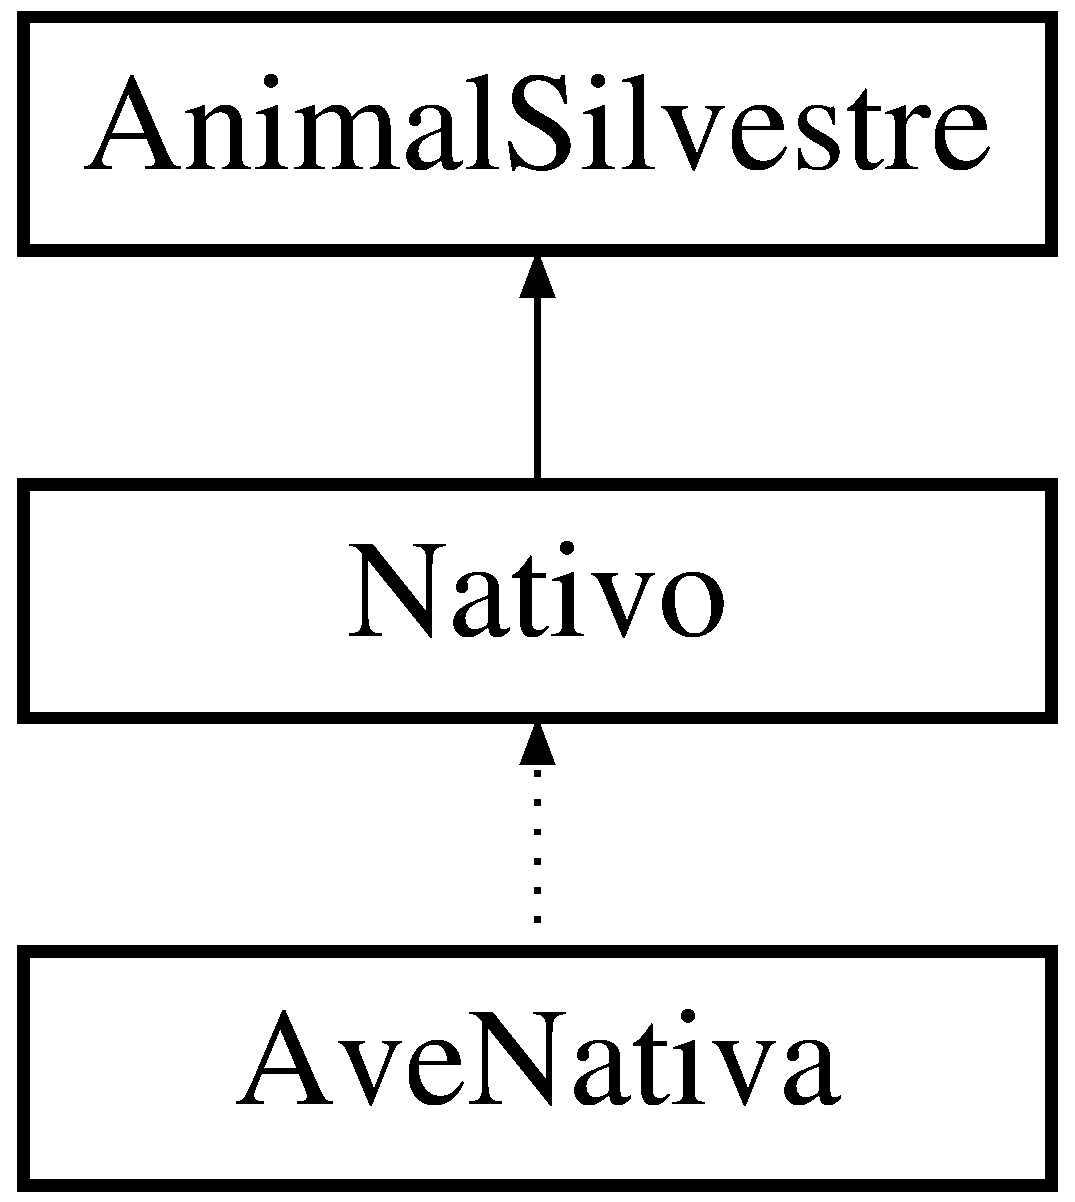
\includegraphics[height=3.000000cm]{classNativo}
\end{center}
\end{figure}
\subsection*{Public Member Functions}
\begin{DoxyCompactItemize}
\item 
\mbox{\Hypertarget{classNativo_af8d9129aa83fdb5fc4956167f13ce251}\label{classNativo_af8d9129aa83fdb5fc4956167f13ce251}} 
{\bfseries Nativo} (std\+::string \+\_\+permissao\+\_\+ibama, std\+::string \+\_\+estado\+\_\+de\+\_\+origem, std\+::string \+\_\+autorizacao)
\item 
\mbox{\Hypertarget{classNativo_af97564a1f971167fdc5d8676e9bcb649}\label{classNativo_af97564a1f971167fdc5d8676e9bcb649}} 
void {\bfseries set\+Autorizacao} (std\+::string \+\_\+autorizacao)
\item 
\mbox{\Hypertarget{classNativo_aff24d9940ac1f8310b55ce1c2b14df98}\label{classNativo_aff24d9940ac1f8310b55ce1c2b14df98}} 
virtual std\+::string {\bfseries get\+Permissao} () const =0
\item 
\mbox{\Hypertarget{classNativo_a83f2b4924bc193ae56637ff5db9627c5}\label{classNativo_a83f2b4924bc193ae56637ff5db9627c5}} 
virtual std\+::string {\bfseries get\+Estado\+De\+Origem} () const =0
\item 
\mbox{\Hypertarget{classNativo_a1518e3beaa33ebd30c318e305961fb2d}\label{classNativo_a1518e3beaa33ebd30c318e305961fb2d}} 
virtual std\+::string {\bfseries get\+Autorizacao} () const =0
\end{DoxyCompactItemize}
\subsection*{Protected Attributes}
\begin{DoxyCompactItemize}
\item 
\mbox{\Hypertarget{classNativo_a7febbf72b864b4b3c348688d21cc74c2}\label{classNativo_a7febbf72b864b4b3c348688d21cc74c2}} 
std\+::string {\bfseries estado\+\_\+de\+\_\+origem}
\item 
\mbox{\Hypertarget{classNativo_a6b1f34afe061f326edd205474b5ae0da}\label{classNativo_a6b1f34afe061f326edd205474b5ae0da}} 
std\+::string {\bfseries autorizacao}
\end{DoxyCompactItemize}


The documentation for this class was generated from the following files\+:\begin{DoxyCompactItemize}
\item 
/home/xsolowingx/\+L\+P1/\+Programas/\+Projeto3/include/\hyperlink{nativo_8h}{nativo.\+h}\item 
/home/xsolowingx/\+L\+P1/\+Programas/\+Projeto3/src/\hyperlink{nativo_8cpp}{nativo.\+cpp}\end{DoxyCompactItemize}

\hypertarget{classReptil}{}\section{Reptil Class Reference}
\label{classReptil}\index{Reptil@{Reptil}}
Inheritance diagram for Reptil\+:\begin{figure}[H]
\begin{center}
\leavevmode
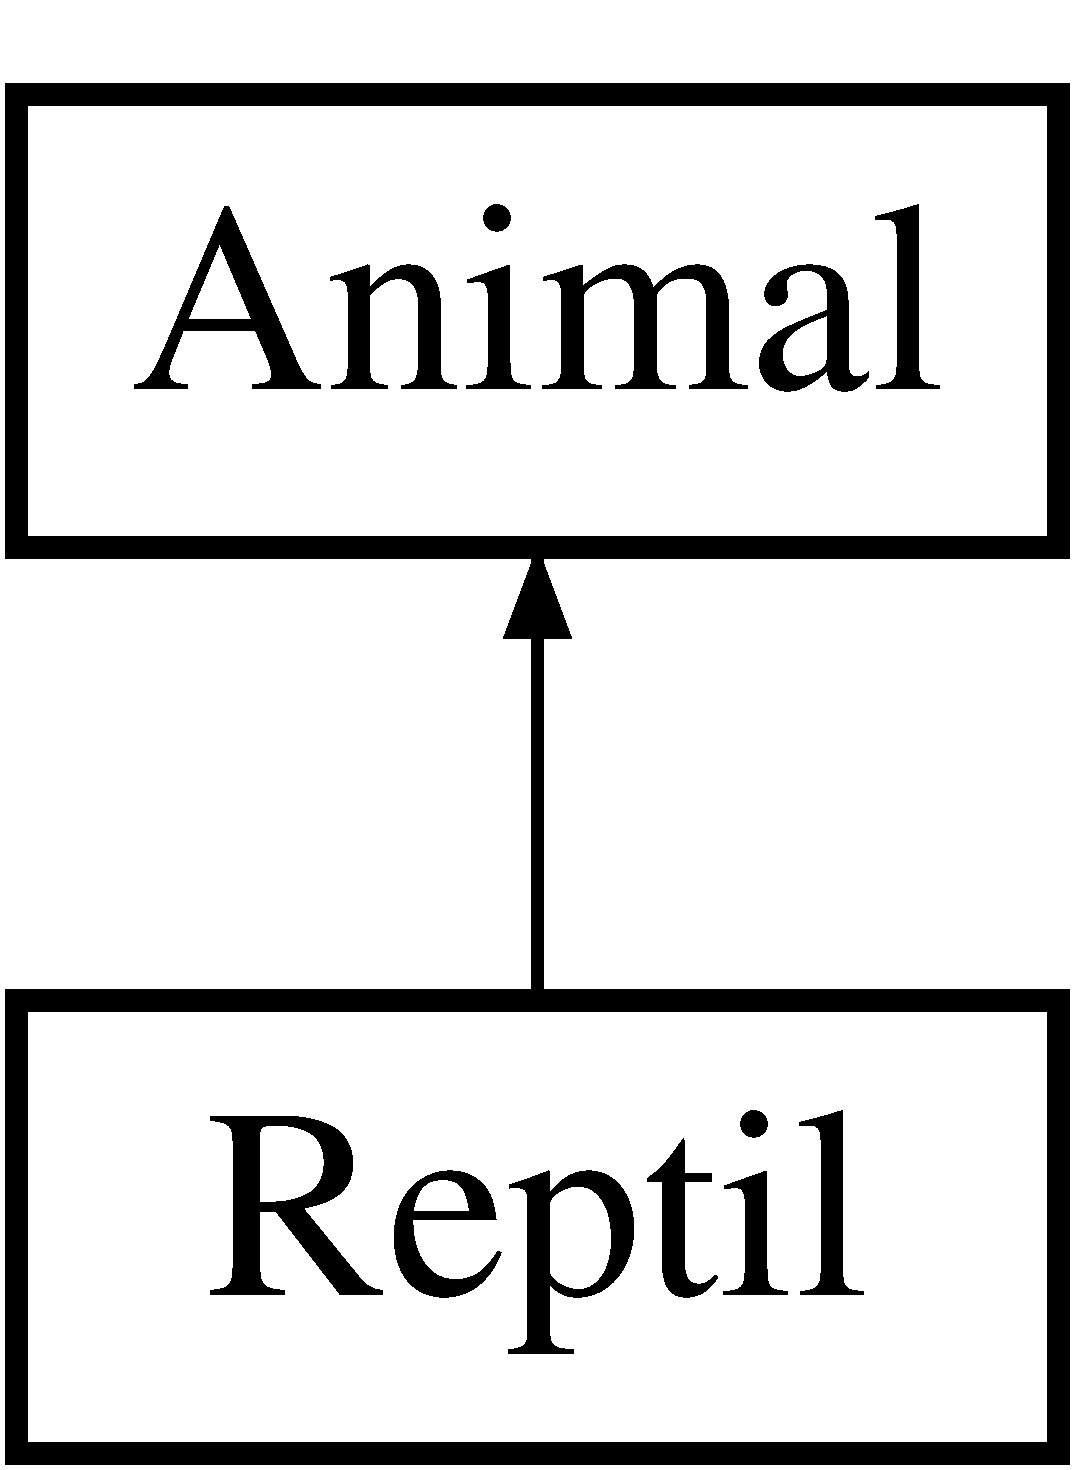
\includegraphics[height=2.000000cm]{classReptil}
\end{center}
\end{figure}
\subsection*{Public Member Functions}
\begin{DoxyCompactItemize}
\item 
\mbox{\Hypertarget{classReptil_aae8f6accbf1eff6e060b011a43349730}\label{classReptil_aae8f6accbf1eff6e060b011a43349730}} 
{\bfseries Reptil} (std\+::string \+\_\+id, std\+::string \+\_\+classe, std\+::string \+\_\+nome\+\_\+especie, std\+::string \+\_\+nome\+\_\+cientifico, char \+\_\+sexo, float \+\_\+tamanho, std\+::string \+\_\+dieta, \hyperlink{classVeterinario}{Veterinario} \&\+\_\+veterinario, \hyperlink{classTratador}{Tratador} \&\+\_\+tratador, std\+::string \+\_\+nome\+\_\+de\+\_\+batismo, bool \+\_\+venenoso, std\+::string \+\_\+tipo\+\_\+veneno)
\item 
\mbox{\Hypertarget{classReptil_aa5e4cd3fa2d94916a3ba5cc20299d3cf}\label{classReptil_aa5e4cd3fa2d94916a3ba5cc20299d3cf}} 
std\+::string {\bfseries get\+Tipo\+Veneno} ()
\item 
\mbox{\Hypertarget{classReptil_a75138aaa91420a9f82ddd39c19ea8b78}\label{classReptil_a75138aaa91420a9f82ddd39c19ea8b78}} 
bool {\bfseries get\+Venenoso} ()
\item 
\mbox{\Hypertarget{classReptil_a8bcbdba3b28482246ec7820f73649aee}\label{classReptil_a8bcbdba3b28482246ec7820f73649aee}} 
std\+::ostream \& {\bfseries print} (std\+::ostream \&o)
\end{DoxyCompactItemize}
\subsection*{Protected Attributes}
\begin{DoxyCompactItemize}
\item 
\mbox{\Hypertarget{classReptil_a7cdfbf53287364cf8f7582cf1f8c3ad6}\label{classReptil_a7cdfbf53287364cf8f7582cf1f8c3ad6}} 
bool {\bfseries venenoso}
\item 
\mbox{\Hypertarget{classReptil_add2a1f28ecb68b69b000ccdfa76b530f}\label{classReptil_add2a1f28ecb68b69b000ccdfa76b530f}} 
std\+::string {\bfseries tipo\+\_\+veneno}
\end{DoxyCompactItemize}


The documentation for this class was generated from the following files\+:\begin{DoxyCompactItemize}
\item 
/home/xsolowingx/\+L\+P1/\+Programas/\+Projeto3/include/\hyperlink{reptil_8h}{reptil.\+h}\item 
/home/xsolowingx/\+L\+P1/\+Programas/\+Projeto3/src/\hyperlink{reptil_8cpp}{reptil.\+cpp}\end{DoxyCompactItemize}

\hypertarget{classTratador}{}\section{Tratador Class Reference}
\label{classTratador}\index{Tratador@{Tratador}}
Inheritance diagram for Tratador\+:\begin{figure}[H]
\begin{center}
\leavevmode
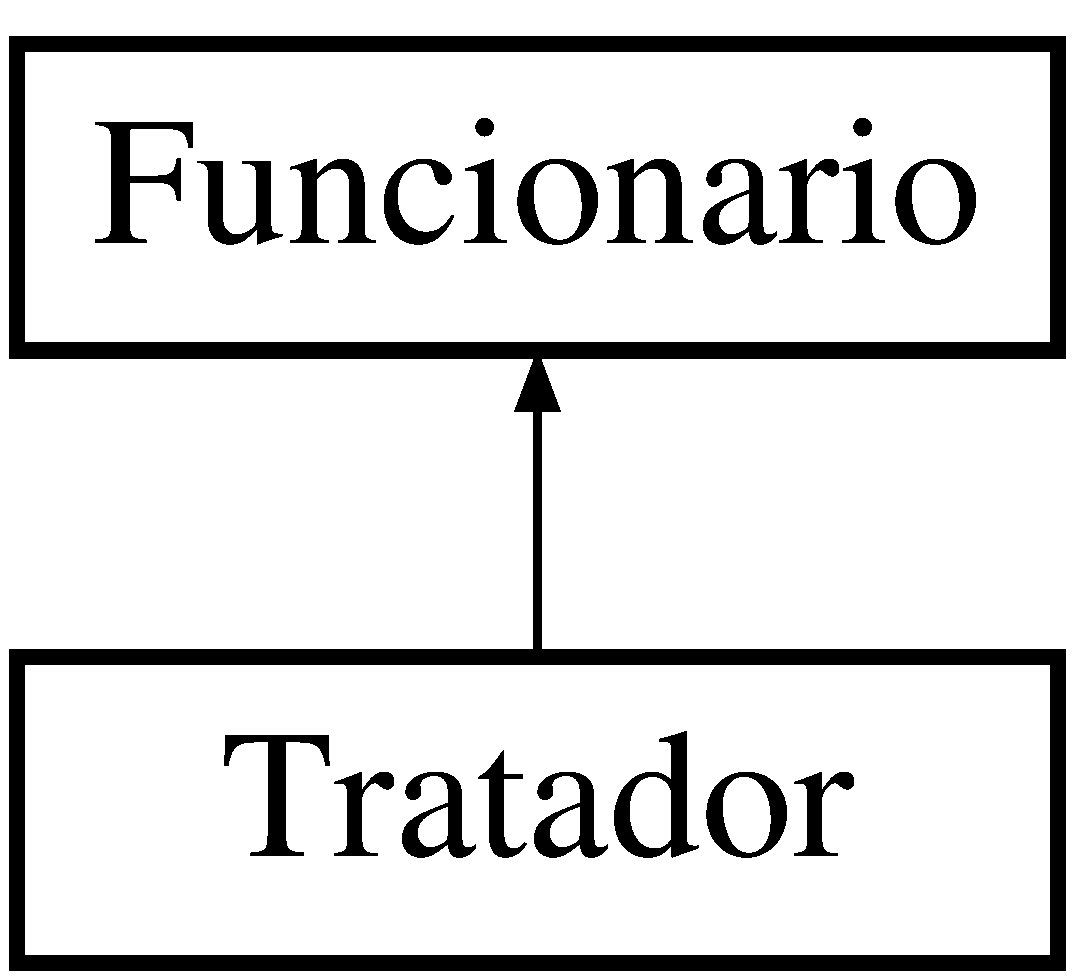
\includegraphics[height=2.000000cm]{classTratador}
\end{center}
\end{figure}
\subsection*{Public Member Functions}
\begin{DoxyCompactItemize}
\item 
\mbox{\Hypertarget{classTratador_ad9e8333c7fb8b232c89744036d08a254}\label{classTratador_ad9e8333c7fb8b232c89744036d08a254}} 
{\bfseries Tratador} (std\+::string \+\_\+id, std\+::string \+\_\+nome, std\+::string \+\_\+cpf, std\+::string \+\_\+idade, std\+::string \+\_\+tipo\+\_\+sanguineo, std\+::string \+\_\+fator\+RH, std\+::string \+\_\+especialidade, std\+::string \+\_\+funcao)
\item 
\mbox{\Hypertarget{classTratador_a835c33d9d4451f425e0dd9e083ee104e}\label{classTratador_a835c33d9d4451f425e0dd9e083ee104e}} 
{\bfseries Tratador} (\hyperlink{classTratador}{Tratador} \&t)
\item 
\mbox{\Hypertarget{classTratador_a21e41c2e6c02a0223af74f5c10ca352f}\label{classTratador_a21e41c2e6c02a0223af74f5c10ca352f}} 
std\+::ostream \& {\bfseries print} (std\+::ostream \&o)
\item 
\mbox{\Hypertarget{classTratador_a336550a0c12a4db6f02d6246beb7440b}\label{classTratador_a336550a0c12a4db6f02d6246beb7440b}} 
std\+::istream \& {\bfseries scan} (std\+::istream \&i)
\item 
\mbox{\Hypertarget{classTratador_aa8dd71720d4b5eaef8fb6dd7f6bb485c}\label{classTratador_aa8dd71720d4b5eaef8fb6dd7f6bb485c}} 
\hyperlink{classTratador}{Tratador} \& {\bfseries operator=} (\hyperlink{classTratador}{Tratador} \&t)
\end{DoxyCompactItemize}
\subsection*{Friends}
\begin{DoxyCompactItemize}
\item 
\mbox{\Hypertarget{classTratador_a80d2acf043be5b18ff7f049821326d3a}\label{classTratador_a80d2acf043be5b18ff7f049821326d3a}} 
std\+::ostream \& {\bfseries operator$<$$<$} (std\+::ostream \&o, \hyperlink{classTratador}{Tratador} \&t)
\end{DoxyCompactItemize}
\subsection*{Additional Inherited Members}


The documentation for this class was generated from the following files\+:\begin{DoxyCompactItemize}
\item 
/home/xsolowingx/\+L\+P1/\+Programas/\+Projeto3/include/\hyperlink{tratador_8h}{tratador.\+h}\item 
/home/xsolowingx/\+L\+P1/\+Programas/\+Projeto3/src/\hyperlink{tratador_8cpp}{tratador.\+cpp}\end{DoxyCompactItemize}

\hypertarget{classVeterinario}{}\section{Veterinario Class Reference}
\label{classVeterinario}\index{Veterinario@{Veterinario}}
Inheritance diagram for Veterinario\+:\begin{figure}[H]
\begin{center}
\leavevmode
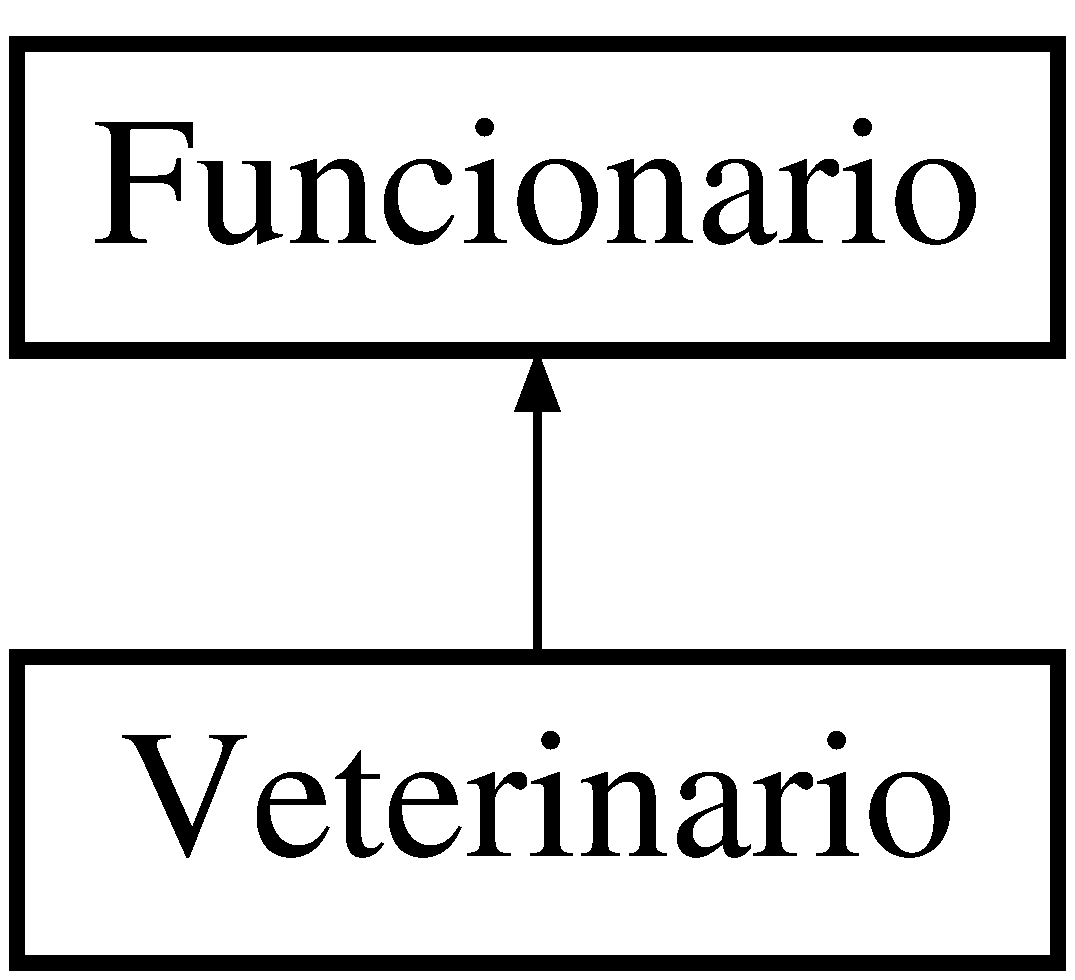
\includegraphics[height=2.000000cm]{classVeterinario}
\end{center}
\end{figure}
\subsection*{Public Member Functions}
\begin{DoxyCompactItemize}
\item 
\mbox{\Hypertarget{classVeterinario_a18edd650b6f5d8c134e30df99f96a20f}\label{classVeterinario_a18edd650b6f5d8c134e30df99f96a20f}} 
{\bfseries Veterinario} (std\+::string \+\_\+id, std\+::string \+\_\+nome, std\+::string \+\_\+cpf, std\+::string \+\_\+idade, std\+::string \+\_\+tipo\+\_\+sanguineo, std\+::string \+\_\+fator\+RH, std\+::string \+\_\+especialidade, std\+::string \+\_\+funcao)
\item 
\mbox{\Hypertarget{classVeterinario_af7a07127569ee82336197f5d1b156081}\label{classVeterinario_af7a07127569ee82336197f5d1b156081}} 
{\bfseries Veterinario} (\hyperlink{classVeterinario}{Veterinario} \&v)
\item 
\mbox{\Hypertarget{classVeterinario_a134317f9b85bd72dcc1d3094fa903e40}\label{classVeterinario_a134317f9b85bd72dcc1d3094fa903e40}} 
std\+::ostream \& {\bfseries print} (std\+::ostream \&o)
\item 
\mbox{\Hypertarget{classVeterinario_ad0909337d5bb3cc79df645cdf2c0af09}\label{classVeterinario_ad0909337d5bb3cc79df645cdf2c0af09}} 
std\+::istream \& {\bfseries scan} (std\+::istream \&i)
\item 
\mbox{\Hypertarget{classVeterinario_ab8f9a3de7aef6e1b26bbcf7e12b3d61b}\label{classVeterinario_ab8f9a3de7aef6e1b26bbcf7e12b3d61b}} 
\hyperlink{classVeterinario}{Veterinario} \& {\bfseries operator=} (\hyperlink{classVeterinario}{Veterinario} \&v)
\end{DoxyCompactItemize}
\subsection*{Friends}
\begin{DoxyCompactItemize}
\item 
\mbox{\Hypertarget{classVeterinario_a62553f6b0a0a3fdd3b7ac1e8b5a9d4d9}\label{classVeterinario_a62553f6b0a0a3fdd3b7ac1e8b5a9d4d9}} 
std\+::ostream \& {\bfseries operator$<$$<$} (std\+::ostream \&o, \hyperlink{classVeterinario}{Veterinario} \&v)
\end{DoxyCompactItemize}
\subsection*{Additional Inherited Members}


The documentation for this class was generated from the following files\+:\begin{DoxyCompactItemize}
\item 
/home/xsolowingx/\+L\+P1/\+Programas/\+Projeto3/include/\hyperlink{veterinario_8h}{veterinario.\+h}\item 
/home/xsolowingx/\+L\+P1/\+Programas/\+Projeto3/src/\hyperlink{veterinario_8cpp}{veterinario.\+cpp}\end{DoxyCompactItemize}

\chapter{File Documentation}
\hypertarget{anfibio_8h}{}\section{/home/xsolowingx/\+L\+P1/\+Programas/\+Projeto3/include/anfibio.h File Reference}
\label{anfibio_8h}\index{/home/xsolowingx/\+L\+P1/\+Programas/\+Projeto3/include/anfibio.\+h@{/home/xsolowingx/\+L\+P1/\+Programas/\+Projeto3/include/anfibio.\+h}}


arquivo que contém as definições da classe \hyperlink{classAnfibio}{Anfibio}  


{\ttfamily \#include \char`\"{}animal.\+h\char`\"{}}\newline
\subsection*{Classes}
\begin{DoxyCompactItemize}
\item 
class \hyperlink{classAnfibio}{Anfibio}
\end{DoxyCompactItemize}


\subsection{Detailed Description}
arquivo que contém as definições da classe \hyperlink{classAnfibio}{Anfibio} 

\begin{DoxySince}{Since}
30/11/2017
\end{DoxySince}
\begin{DoxyAuthor}{Author}
Matheus de Jesus Leandro de Medeiros 
\end{DoxyAuthor}
\begin{DoxyDate}{Date}
08/12/17 
\end{DoxyDate}

\hypertarget{animal_8h}{}\section{/home/xsolowingx/\+L\+P1/\+Programas/\+Projeto3/include/animal.h File Reference}
\label{animal_8h}\index{/home/xsolowingx/\+L\+P1/\+Programas/\+Projeto3/include/animal.\+h@{/home/xsolowingx/\+L\+P1/\+Programas/\+Projeto3/include/animal.\+h}}


arquivo que contém as definições da classe \hyperlink{classAnimal}{Animal}  


{\ttfamily \#include \char`\"{}veterinario.\+h\char`\"{}}\newline
{\ttfamily \#include \char`\"{}tratador.\+h\char`\"{}}\newline
\subsection*{Classes}
\begin{DoxyCompactItemize}
\item 
class \hyperlink{classAnimal}{Animal}
\end{DoxyCompactItemize}


\subsection{Detailed Description}
arquivo que contém as definições da classe \hyperlink{classAnimal}{Animal} 

\begin{DoxySince}{Since}
30/11/2017
\end{DoxySince}
\begin{DoxyAuthor}{Author}
Matheus de Jesus Leandro de Medeiros 
\end{DoxyAuthor}
\begin{DoxyDate}{Date}
08/12/17 
\end{DoxyDate}

\hypertarget{animalSilvestre_8h}{}\section{/home/xsolowingx/\+L\+P1/\+Programas/\+Projeto3/include/animal\+Silvestre.h File Reference}
\label{animalSilvestre_8h}\index{/home/xsolowingx/\+L\+P1/\+Programas/\+Projeto3/include/animal\+Silvestre.\+h@{/home/xsolowingx/\+L\+P1/\+Programas/\+Projeto3/include/animal\+Silvestre.\+h}}


arquivo que contém as definições da classe \hyperlink{classAnimalSilvestre}{Animal\+Silvestre}  


{\ttfamily \#include $<$string$>$}\newline
\subsection*{Classes}
\begin{DoxyCompactItemize}
\item 
class \hyperlink{classAnimalSilvestre}{Animal\+Silvestre}
\end{DoxyCompactItemize}


\subsection{Detailed Description}
arquivo que contém as definições da classe \hyperlink{classAnimalSilvestre}{Animal\+Silvestre} 

\begin{DoxySince}{Since}
30/11/2017
\end{DoxySince}
\begin{DoxyAuthor}{Author}
Matheus de Jesus Leandro de Medeiros 
\end{DoxyAuthor}
\begin{DoxyDate}{Date}
08/12/17 
\end{DoxyDate}

\hypertarget{ave_8h}{}\section{/home/xsolowingx/\+L\+P1/\+Programas/\+Projeto3/include/ave.h File Reference}
\label{ave_8h}\index{/home/xsolowingx/\+L\+P1/\+Programas/\+Projeto3/include/ave.\+h@{/home/xsolowingx/\+L\+P1/\+Programas/\+Projeto3/include/ave.\+h}}


arquivo que contém as definições da classe \hyperlink{classAve}{Ave}  


{\ttfamily \#include \char`\"{}animal.\+h\char`\"{}}\newline
\subsection*{Classes}
\begin{DoxyCompactItemize}
\item 
class \hyperlink{classAve}{Ave}
\end{DoxyCompactItemize}


\subsection{Detailed Description}
arquivo que contém as definições da classe \hyperlink{classAve}{Ave} 

\begin{DoxySince}{Since}
30/11/2017
\end{DoxySince}
\begin{DoxyAuthor}{Author}
Matheus de Jesus Leandro de Medeiros 
\end{DoxyAuthor}
\begin{DoxyDate}{Date}
08/12/17 
\end{DoxyDate}

\hypertarget{aveExotica_8h}{}\section{/home/xsolowingx/\+L\+P1/\+Programas/\+Projeto3/include/ave\+Exotica.h File Reference}
\label{aveExotica_8h}\index{/home/xsolowingx/\+L\+P1/\+Programas/\+Projeto3/include/ave\+Exotica.\+h@{/home/xsolowingx/\+L\+P1/\+Programas/\+Projeto3/include/ave\+Exotica.\+h}}


arquivo que contém as definições da classe \hyperlink{classAveExotica}{Ave\+Exotica}  


{\ttfamily \#include \char`\"{}ave.\+h\char`\"{}}\newline
{\ttfamily \#include \char`\"{}exotico.\+h\char`\"{}}\newline
\subsection*{Classes}
\begin{DoxyCompactItemize}
\item 
class \hyperlink{classAveExotica}{Ave\+Exotica}
\end{DoxyCompactItemize}


\subsection{Detailed Description}
arquivo que contém as definições da classe \hyperlink{classAveExotica}{Ave\+Exotica} 

\begin{DoxySince}{Since}
30/11/2017
\end{DoxySince}
\begin{DoxyAuthor}{Author}
Matheus de Jesus Leandro de Medeiros 
\end{DoxyAuthor}
\begin{DoxyDate}{Date}
08/12/17 
\end{DoxyDate}

\hypertarget{aveNativa_8h}{}\section{/home/xsolowingx/\+L\+P1/\+Programas/\+Projeto3/include/ave\+Nativa.h File Reference}
\label{aveNativa_8h}\index{/home/xsolowingx/\+L\+P1/\+Programas/\+Projeto3/include/ave\+Nativa.\+h@{/home/xsolowingx/\+L\+P1/\+Programas/\+Projeto3/include/ave\+Nativa.\+h}}


arquivo que contém as definições da classe \hyperlink{classAveNativa}{Ave\+Nativa}  


{\ttfamily \#include \char`\"{}ave.\+h\char`\"{}}\newline
{\ttfamily \#include \char`\"{}nativo.\+h\char`\"{}}\newline
\subsection*{Classes}
\begin{DoxyCompactItemize}
\item 
class \hyperlink{classAveNativa}{Ave\+Nativa}
\end{DoxyCompactItemize}


\subsection{Detailed Description}
arquivo que contém as definições da classe \hyperlink{classAveNativa}{Ave\+Nativa} 

\begin{DoxySince}{Since}
30/11/2017
\end{DoxySince}
\begin{DoxyAuthor}{Author}
Matheus de Jesus Leandro de Medeiros 
\end{DoxyAuthor}
\begin{DoxyDate}{Date}
08/12/17 
\end{DoxyDate}

\hypertarget{classes_8h}{}\section{/home/xsolowingx/\+L\+P1/\+Programas/\+Projeto3/include/classes.h File Reference}
\label{classes_8h}\index{/home/xsolowingx/\+L\+P1/\+Programas/\+Projeto3/include/classes.\+h@{/home/xsolowingx/\+L\+P1/\+Programas/\+Projeto3/include/classes.\+h}}


arquivo que contém todas as bibliotecas com classes inclusas.  


{\ttfamily \#include \char`\"{}funcionario.\+h\char`\"{}}\newline
{\ttfamily \#include \char`\"{}veterinario.\+h\char`\"{}}\newline
{\ttfamily \#include \char`\"{}tratador.\+h\char`\"{}}\newline
{\ttfamily \#include \char`\"{}animal.\+h\char`\"{}}\newline
{\ttfamily \#include \char`\"{}anfibio.\+h\char`\"{}}\newline
{\ttfamily \#include \char`\"{}reptil.\+h\char`\"{}}\newline
{\ttfamily \#include \char`\"{}mamifero.\+h\char`\"{}}\newline
{\ttfamily \#include \char`\"{}ave.\+h\char`\"{}}\newline
{\ttfamily \#include \char`\"{}animal\+Silvestre.\+h\char`\"{}}\newline
{\ttfamily \#include \char`\"{}nativo.\+h\char`\"{}}\newline
{\ttfamily \#include \char`\"{}exotico.\+h\char`\"{}}\newline
{\ttfamily \#include \char`\"{}ave\+Nativa.\+h\char`\"{}}\newline
{\ttfamily \#include \char`\"{}ave\+Exotica.\+h\char`\"{}}\newline
{\ttfamily \#include \char`\"{}excecoes.\+h\char`\"{}}\newline


\subsection{Detailed Description}
arquivo que contém todas as bibliotecas com classes inclusas. 

\begin{DoxySince}{Since}
30/11/2017
\end{DoxySince}
\begin{DoxyAuthor}{Author}
Matheus de Jesus Leandro de Medeiros 
\end{DoxyAuthor}
\begin{DoxyDate}{Date}
08/12/17 
\end{DoxyDate}

\hypertarget{excecoes_8h}{}\section{/home/xsolowingx/\+L\+P1/\+Programas/\+Projeto3/include/excecoes.h File Reference}
\label{excecoes_8h}\index{/home/xsolowingx/\+L\+P1/\+Programas/\+Projeto3/include/excecoes.\+h@{/home/xsolowingx/\+L\+P1/\+Programas/\+Projeto3/include/excecoes.\+h}}


arquivo que contém as definições das classes com as possíveis Exceções.  


{\ttfamily \#include $<$exception$>$}\newline
{\ttfamily \#include $<$stdexcept$>$}\newline
{\ttfamily \#include $<$string$>$}\newline
\subsection*{Classes}
\begin{DoxyCompactItemize}
\item 
class \hyperlink{classErroAoAbrirArquivo}{Erro\+Ao\+Abrir\+Arquivo}
\item 
class \hyperlink{classErroAoTentarLerDados}{Erro\+Ao\+Tentar\+Ler\+Dados}
\end{DoxyCompactItemize}


\subsection{Detailed Description}
arquivo que contém as definições das classes com as possíveis Exceções. 

\begin{DoxySince}{Since}
30/11/2017
\end{DoxySince}
\begin{DoxyAuthor}{Author}
Matheus de Jesus Leandro de Medeiros 
\end{DoxyAuthor}
\begin{DoxyDate}{Date}
08/12/17 
\end{DoxyDate}

\hypertarget{exotico_8h}{}\section{/home/xsolowingx/\+L\+P1/\+Programas/\+Projeto3/include/exotico.h File Reference}
\label{exotico_8h}\index{/home/xsolowingx/\+L\+P1/\+Programas/\+Projeto3/include/exotico.\+h@{/home/xsolowingx/\+L\+P1/\+Programas/\+Projeto3/include/exotico.\+h}}


arquivo que contém as definições da classe \hyperlink{classExotico}{Exotico}  


{\ttfamily \#include \char`\"{}animal\+Silvestre.\+h\char`\"{}}\newline
\subsection*{Classes}
\begin{DoxyCompactItemize}
\item 
class \hyperlink{classExotico}{Exotico}
\end{DoxyCompactItemize}


\subsection{Detailed Description}
arquivo que contém as definições da classe \hyperlink{classExotico}{Exotico} 

\begin{DoxySince}{Since}
30/11/2017
\end{DoxySince}
\begin{DoxyAuthor}{Author}
Matheus de Jesus Leandro de Medeiros 
\end{DoxyAuthor}
\begin{DoxyDate}{Date}
08/12/17 
\end{DoxyDate}

\hypertarget{funcionario_8h}{}\section{/home/xsolowingx/\+L\+P1/\+Programas/\+Projeto3/include/funcionario.h File Reference}
\label{funcionario_8h}\index{/home/xsolowingx/\+L\+P1/\+Programas/\+Projeto3/include/funcionario.\+h@{/home/xsolowingx/\+L\+P1/\+Programas/\+Projeto3/include/funcionario.\+h}}


arquivo que contém as definições da classe \hyperlink{classFuncionario}{Funcionario}  


{\ttfamily \#include $<$string$>$}\newline
{\ttfamily \#include $<$ostream$>$}\newline
{\ttfamily \#include $<$istream$>$}\newline
\subsection*{Classes}
\begin{DoxyCompactItemize}
\item 
class \hyperlink{classFuncionario}{Funcionario}
\end{DoxyCompactItemize}


\subsection{Detailed Description}
arquivo que contém as definições da classe \hyperlink{classFuncionario}{Funcionario} 

\begin{DoxySince}{Since}
30/11/2017
\end{DoxySince}
\begin{DoxyAuthor}{Author}
Matheus de Jesus Leandro de Medeiros 
\end{DoxyAuthor}
\begin{DoxyDate}{Date}
08/12/17 
\end{DoxyDate}

\hypertarget{funcoes_8h}{}\section{/home/xsolowingx/\+L\+P1/\+Programas/\+Projeto3/include/funcoes.h File Reference}
\label{funcoes_8h}\index{/home/xsolowingx/\+L\+P1/\+Programas/\+Projeto3/include/funcoes.\+h@{/home/xsolowingx/\+L\+P1/\+Programas/\+Projeto3/include/funcoes.\+h}}


arquivo onde contém as definições das funções auxiliares do programa Petfera  


{\ttfamily \#include $<$fstream$>$}\newline
{\ttfamily \#include $<$memory$>$}\newline
{\ttfamily \#include $<$vector$>$}\newline
{\ttfamily \#include \char`\"{}classes.\+h\char`\"{}}\newline
\subsection*{Functions}
\begin{DoxyCompactItemize}
\item 
bool \hyperlink{funcoes_8h_a757f27dfa9fc7a46f59900cbe55af76a}{ler\+Funcionarios} (std\+::ifstream \&ifs, std\+::vector$<$ std\+::shared\+\_\+ptr$<$ \hyperlink{classFuncionario}{Funcionario} $>$$>$ funcs)
\end{DoxyCompactItemize}


\subsection{Detailed Description}
arquivo onde contém as definições das funções auxiliares do programa Petfera 

\begin{DoxySince}{Since}
30/11/2017
\end{DoxySince}
\begin{DoxyAuthor}{Author}
Matheus de Jesus Leandro de Medeiros 
\end{DoxyAuthor}
\begin{DoxyDate}{Date}
08/12/17 
\end{DoxyDate}


\subsection{Function Documentation}
\mbox{\Hypertarget{funcoes_8h_a757f27dfa9fc7a46f59900cbe55af76a}\label{funcoes_8h_a757f27dfa9fc7a46f59900cbe55af76a}} 
\index{funcoes.\+h@{funcoes.\+h}!ler\+Funcionarios@{ler\+Funcionarios}}
\index{ler\+Funcionarios@{ler\+Funcionarios}!funcoes.\+h@{funcoes.\+h}}
\subsubsection{\texorpdfstring{ler\+Funcionarios()}{lerFuncionarios()}}
{\footnotesize\ttfamily bool ler\+Funcionarios (\begin{DoxyParamCaption}\item[{std\+::ifstream \&}]{ifs,  }\item[{std\+::vector$<$ std\+::shared\+\_\+ptr$<$ \hyperlink{classFuncionario}{Funcionario} $>$$>$}]{funcs }\end{DoxyParamCaption})}


\begin{DoxyParams}{Parameters}
{\em ifs} & um arquivo de leitura \\
\hline
{\em funcs} & vector de shared\+\_\+ptrs\\
\hline
\end{DoxyParams}
função que lê os dados dos funcionários no arquivo funcionarios.\+csv, inicialmente ela adiciona um objeto da classe \hyperlink{classTratador}{Tratador} ou \hyperlink{classVeterinario}{Veterinario} à um vetor de Funcionários, mas a posteriori, ela iria adicionar à um \char`\"{}map\char`\"{}.

\begin{DoxyReturn}{Returns}
\{ true ou false \} 
\end{DoxyReturn}

\hypertarget{mamifero_8h}{}\section{/home/xsolowingx/\+L\+P1/\+Programas/\+Projeto3/include/mamifero.h File Reference}
\label{mamifero_8h}\index{/home/xsolowingx/\+L\+P1/\+Programas/\+Projeto3/include/mamifero.\+h@{/home/xsolowingx/\+L\+P1/\+Programas/\+Projeto3/include/mamifero.\+h}}


arquivo que contém as definições da classe \hyperlink{classMamifero}{Mamifero}  


{\ttfamily \#include \char`\"{}animal.\+h\char`\"{}}\newline
\subsection*{Classes}
\begin{DoxyCompactItemize}
\item 
class \hyperlink{classMamifero}{Mamifero}
\end{DoxyCompactItemize}


\subsection{Detailed Description}
arquivo que contém as definições da classe \hyperlink{classMamifero}{Mamifero} 

\begin{DoxySince}{Since}
30/11/2017
\end{DoxySince}
\begin{DoxyAuthor}{Author}
Matheus de Jesus Leandro de Medeiros 
\end{DoxyAuthor}
\begin{DoxyDate}{Date}
08/12/17 
\end{DoxyDate}

\hypertarget{nativo_8h}{}\section{/home/xsolowingx/\+L\+P1/\+Programas/\+Projeto3/include/nativo.h File Reference}
\label{nativo_8h}\index{/home/xsolowingx/\+L\+P1/\+Programas/\+Projeto3/include/nativo.\+h@{/home/xsolowingx/\+L\+P1/\+Programas/\+Projeto3/include/nativo.\+h}}


arquivo que contém as definições da classe \hyperlink{classNativo}{Nativo}  


{\ttfamily \#include \char`\"{}animal\+Silvestre.\+h\char`\"{}}\newline
\subsection*{Classes}
\begin{DoxyCompactItemize}
\item 
class \hyperlink{classNativo}{Nativo}
\end{DoxyCompactItemize}


\subsection{Detailed Description}
arquivo que contém as definições da classe \hyperlink{classNativo}{Nativo} 

\begin{DoxySince}{Since}
30/11/2017
\end{DoxySince}
\begin{DoxyAuthor}{Author}
Matheus de Jesus Leandro de Medeiros 
\end{DoxyAuthor}
\begin{DoxyDate}{Date}
08/12/17 
\end{DoxyDate}

\hypertarget{reptil_8h}{}\section{/home/xsolowingx/\+L\+P1/\+Programas/\+Projeto3/include/reptil.h File Reference}
\label{reptil_8h}\index{/home/xsolowingx/\+L\+P1/\+Programas/\+Projeto3/include/reptil.\+h@{/home/xsolowingx/\+L\+P1/\+Programas/\+Projeto3/include/reptil.\+h}}


arquivo que contém as definições da classe \hyperlink{classReptil}{Reptil}  


{\ttfamily \#include \char`\"{}animal.\+h\char`\"{}}\newline
\subsection*{Classes}
\begin{DoxyCompactItemize}
\item 
class \hyperlink{classReptil}{Reptil}
\end{DoxyCompactItemize}


\subsection{Detailed Description}
arquivo que contém as definições da classe \hyperlink{classReptil}{Reptil} 

\begin{DoxySince}{Since}
30/11/2017
\end{DoxySince}
\begin{DoxyAuthor}{Author}
Matheus de Jesus Leandro de Medeiros 
\end{DoxyAuthor}
\begin{DoxyDate}{Date}
08/12/17 
\end{DoxyDate}

\hypertarget{tratador_8h}{}\section{/home/xsolowingx/\+L\+P1/\+Programas/\+Projeto3/include/tratador.h File Reference}
\label{tratador_8h}\index{/home/xsolowingx/\+L\+P1/\+Programas/\+Projeto3/include/tratador.\+h@{/home/xsolowingx/\+L\+P1/\+Programas/\+Projeto3/include/tratador.\+h}}


arquivo que contém as definições da classe \hyperlink{classTratador}{Tratador}  


{\ttfamily \#include \char`\"{}funcionario.\+h\char`\"{}}\newline
\subsection*{Classes}
\begin{DoxyCompactItemize}
\item 
class \hyperlink{classTratador}{Tratador}
\end{DoxyCompactItemize}


\subsection{Detailed Description}
arquivo que contém as definições da classe \hyperlink{classTratador}{Tratador} 

\begin{DoxySince}{Since}
30/11/2017
\end{DoxySince}
\begin{DoxyAuthor}{Author}
Matheus de Jesus Leandro de Medeiros 
\end{DoxyAuthor}
\begin{DoxyDate}{Date}
08/12/17 
\end{DoxyDate}

\hypertarget{veterinario_8h}{}\section{/home/xsolowingx/\+L\+P1/\+Programas/\+Projeto3/include/veterinario.h File Reference}
\label{veterinario_8h}\index{/home/xsolowingx/\+L\+P1/\+Programas/\+Projeto3/include/veterinario.\+h@{/home/xsolowingx/\+L\+P1/\+Programas/\+Projeto3/include/veterinario.\+h}}


arquivo que contém as definições da classe \hyperlink{classVeterinario}{Veterinario}  


{\ttfamily \#include \char`\"{}funcionario.\+h\char`\"{}}\newline
\subsection*{Classes}
\begin{DoxyCompactItemize}
\item 
class \hyperlink{classVeterinario}{Veterinario}
\end{DoxyCompactItemize}


\subsection{Detailed Description}
arquivo que contém as definições da classe \hyperlink{classVeterinario}{Veterinario} 

\begin{DoxySince}{Since}
30/11/2017
\end{DoxySince}
\begin{DoxyAuthor}{Author}
Matheus de Jesus Leandro de Medeiros 
\end{DoxyAuthor}
\begin{DoxyDate}{Date}
08/12/17 
\end{DoxyDate}

\hypertarget{anfibio_8cpp}{}\section{/home/xsolowingx/\+L\+P1/\+Programas/\+Projeto3/src/anfibio.cpp File Reference}
\label{anfibio_8cpp}\index{/home/xsolowingx/\+L\+P1/\+Programas/\+Projeto3/src/anfibio.\+cpp@{/home/xsolowingx/\+L\+P1/\+Programas/\+Projeto3/src/anfibio.\+cpp}}


arquivo que contém as implementações da classe \hyperlink{classAnfibio}{Anfibio}  


{\ttfamily \#include \char`\"{}anfibio.\+h\char`\"{}}\newline


\subsection{Detailed Description}
arquivo que contém as implementações da classe \hyperlink{classAnfibio}{Anfibio} 

\begin{DoxySince}{Since}
30/11/2017
\end{DoxySince}
\begin{DoxyAuthor}{Author}
Matheus de Jesus Leandro de Medeiros 
\end{DoxyAuthor}
\begin{DoxyDate}{Date}
08/12/17 
\end{DoxyDate}

\hypertarget{animal_8cpp}{}\section{/home/xsolowingx/\+L\+P1/\+Programas/\+Projeto3/src/animal.cpp File Reference}
\label{animal_8cpp}\index{/home/xsolowingx/\+L\+P1/\+Programas/\+Projeto3/src/animal.\+cpp@{/home/xsolowingx/\+L\+P1/\+Programas/\+Projeto3/src/animal.\+cpp}}


arquivo que contém as implementações da classe \hyperlink{classAnimal}{Animal}  


{\ttfamily \#include \char`\"{}animal.\+h\char`\"{}}\newline
\subsection*{Functions}
\begin{DoxyCompactItemize}
\item 
\mbox{\Hypertarget{animal_8cpp_a60e87f6bdfb739354180c27be7186c0a}\label{animal_8cpp_a60e87f6bdfb739354180c27be7186c0a}} 
std\+::ostream \& {\bfseries operator$<$$<$} (std\+::ostream \&o, \hyperlink{classAnimal}{Animal} \&a)
\end{DoxyCompactItemize}


\subsection{Detailed Description}
arquivo que contém as implementações da classe \hyperlink{classAnimal}{Animal} 

\begin{DoxySince}{Since}
30/11/2017
\end{DoxySince}
\begin{DoxyAuthor}{Author}
Matheus de Jesus Leandro de Medeiros 
\end{DoxyAuthor}
\begin{DoxyDate}{Date}
08/12/17 
\end{DoxyDate}

\hypertarget{animalSilvestre_8cpp}{}\section{/home/xsolowingx/\+L\+P1/\+Programas/\+Projeto3/src/animal\+Silvestre.cpp File Reference}
\label{animalSilvestre_8cpp}\index{/home/xsolowingx/\+L\+P1/\+Programas/\+Projeto3/src/animal\+Silvestre.\+cpp@{/home/xsolowingx/\+L\+P1/\+Programas/\+Projeto3/src/animal\+Silvestre.\+cpp}}


arquivo que contém as implementações da classe \hyperlink{classAnimalSilvestre}{Animal\+Silvestre}  


{\ttfamily \#include \char`\"{}animal\+Silvestre.\+h\char`\"{}}\newline


\subsection{Detailed Description}
arquivo que contém as implementações da classe \hyperlink{classAnimalSilvestre}{Animal\+Silvestre} 

\begin{DoxySince}{Since}
30/11/2017
\end{DoxySince}
\begin{DoxyAuthor}{Author}
Matheus de Jesus Leandro de Medeiros 
\end{DoxyAuthor}
\begin{DoxyDate}{Date}
08/12/17 
\end{DoxyDate}

\hypertarget{ave_8cpp}{}\section{/home/xsolowingx/\+L\+P1/\+Programas/\+Projeto3/src/ave.cpp File Reference}
\label{ave_8cpp}\index{/home/xsolowingx/\+L\+P1/\+Programas/\+Projeto3/src/ave.\+cpp@{/home/xsolowingx/\+L\+P1/\+Programas/\+Projeto3/src/ave.\+cpp}}


arquivo que contém as implementações da classe \hyperlink{classAve}{Ave}  


{\ttfamily \#include \char`\"{}ave.\+h\char`\"{}}\newline


\subsection{Detailed Description}
arquivo que contém as implementações da classe \hyperlink{classAve}{Ave} 

\begin{DoxySince}{Since}
30/11/2017
\end{DoxySince}
\begin{DoxyAuthor}{Author}
Matheus de Jesus Leandro de Medeiros 
\end{DoxyAuthor}
\begin{DoxyDate}{Date}
08/12/17 
\end{DoxyDate}

\hypertarget{aveExotica_8cpp}{}\section{/home/xsolowingx/\+L\+P1/\+Programas/\+Projeto3/src/ave\+Exotica.cpp File Reference}
\label{aveExotica_8cpp}\index{/home/xsolowingx/\+L\+P1/\+Programas/\+Projeto3/src/ave\+Exotica.\+cpp@{/home/xsolowingx/\+L\+P1/\+Programas/\+Projeto3/src/ave\+Exotica.\+cpp}}


arquivo que contém as implementações da classe \hyperlink{classAveExotica}{Ave\+Exotica}  


{\ttfamily \#include \char`\"{}ave\+Exotica.\+h\char`\"{}}\newline


\subsection{Detailed Description}
arquivo que contém as implementações da classe \hyperlink{classAveExotica}{Ave\+Exotica} 

\begin{DoxySince}{Since}
30/11/2017
\end{DoxySince}
\begin{DoxyAuthor}{Author}
Matheus de Jesus Leandro de Medeiros 
\end{DoxyAuthor}
\begin{DoxyDate}{Date}
08/12/17 
\end{DoxyDate}

\hypertarget{aveNativa_8cpp}{}\section{/home/xsolowingx/\+L\+P1/\+Programas/\+Projeto3/src/ave\+Nativa.cpp File Reference}
\label{aveNativa_8cpp}\index{/home/xsolowingx/\+L\+P1/\+Programas/\+Projeto3/src/ave\+Nativa.\+cpp@{/home/xsolowingx/\+L\+P1/\+Programas/\+Projeto3/src/ave\+Nativa.\+cpp}}


arquivo que contém as implementações da classe \hyperlink{classAveNativa}{Ave\+Nativa}  


{\ttfamily \#include \char`\"{}ave\+Nativa.\+h\char`\"{}}\newline


\subsection{Detailed Description}
arquivo que contém as implementações da classe \hyperlink{classAveNativa}{Ave\+Nativa} 

\begin{DoxySince}{Since}
30/11/2017
\end{DoxySince}
\begin{DoxyAuthor}{Author}
Matheus de Jesus Leandro de Medeiros 
\end{DoxyAuthor}
\begin{DoxyDate}{Date}
08/12/17 
\end{DoxyDate}

\hypertarget{excecoes_8cpp}{}\section{/home/xsolowingx/\+L\+P1/\+Programas/\+Projeto3/src/excecoes.cpp File Reference}
\label{excecoes_8cpp}\index{/home/xsolowingx/\+L\+P1/\+Programas/\+Projeto3/src/excecoes.\+cpp@{/home/xsolowingx/\+L\+P1/\+Programas/\+Projeto3/src/excecoes.\+cpp}}


arquivo que contém as implementações das classes de Exceções  


{\ttfamily \#include \char`\"{}excecoes.\+h\char`\"{}}\newline


\subsection{Detailed Description}
arquivo que contém as implementações das classes de Exceções 

\begin{DoxySince}{Since}
30/11/2017
\end{DoxySince}
\begin{DoxyAuthor}{Author}
Matheus de Jesus Leandro de Medeiros 
\end{DoxyAuthor}
\begin{DoxyDate}{Date}
08/12/17 
\end{DoxyDate}

\hypertarget{exotico_8cpp}{}\section{/home/xsolowingx/\+L\+P1/\+Programas/\+Projeto3/src/exotico.cpp File Reference}
\label{exotico_8cpp}\index{/home/xsolowingx/\+L\+P1/\+Programas/\+Projeto3/src/exotico.\+cpp@{/home/xsolowingx/\+L\+P1/\+Programas/\+Projeto3/src/exotico.\+cpp}}


arquivo que contém as implementações da classe \hyperlink{classExotico}{Exotico}  


{\ttfamily \#include \char`\"{}exotico.\+h\char`\"{}}\newline


\subsection{Detailed Description}
arquivo que contém as implementações da classe \hyperlink{classExotico}{Exotico} 

\begin{DoxySince}{Since}
30/11/2017
\end{DoxySince}
\begin{DoxyAuthor}{Author}
Matheus de Jesus Leandro de Medeiros 
\end{DoxyAuthor}
\begin{DoxyDate}{Date}
08/12/17 
\end{DoxyDate}

\hypertarget{funcionario_8cpp}{}\section{/home/xsolowingx/\+L\+P1/\+Programas/\+Projeto3/src/funcionario.cpp File Reference}
\label{funcionario_8cpp}\index{/home/xsolowingx/\+L\+P1/\+Programas/\+Projeto3/src/funcionario.\+cpp@{/home/xsolowingx/\+L\+P1/\+Programas/\+Projeto3/src/funcionario.\+cpp}}


arquivo que contém as implementações da classe \hyperlink{classFuncionario}{Funcionario}  


{\ttfamily \#include \char`\"{}funcionario.\+h\char`\"{}}\newline
\subsection*{Functions}
\begin{DoxyCompactItemize}
\item 
\mbox{\Hypertarget{funcionario_8cpp_a2bb1f75049d15717556f551e25057e93}\label{funcionario_8cpp_a2bb1f75049d15717556f551e25057e93}} 
std\+::istream \& {\bfseries operator$>$$>$} (std\+::istream \&i, \hyperlink{classFuncionario}{Funcionario} \&f)
\item 
\mbox{\Hypertarget{funcionario_8cpp_abdee4494d45e2c0bb334c7ad2a9411c9}\label{funcionario_8cpp_abdee4494d45e2c0bb334c7ad2a9411c9}} 
std\+::ostream \& {\bfseries operator$<$$<$} (std\+::ostream \&o, \hyperlink{classFuncionario}{Funcionario} \&f)
\end{DoxyCompactItemize}


\subsection{Detailed Description}
arquivo que contém as implementações da classe \hyperlink{classFuncionario}{Funcionario} 

\begin{DoxySince}{Since}
30/11/2017
\end{DoxySince}
\begin{DoxyAuthor}{Author}
Matheus de Jesus Leandro de Medeiros 
\end{DoxyAuthor}
\begin{DoxyDate}{Date}
08/12/17 
\end{DoxyDate}

\hypertarget{funcoes_8cpp}{}\section{/home/xsolowingx/\+L\+P1/\+Programas/\+Projeto3/src/funcoes.cpp File Reference}
\label{funcoes_8cpp}\index{/home/xsolowingx/\+L\+P1/\+Programas/\+Projeto3/src/funcoes.\+cpp@{/home/xsolowingx/\+L\+P1/\+Programas/\+Projeto3/src/funcoes.\+cpp}}


arquivo onde contém as implementações das funções auxiliares do programa Petfera  


{\ttfamily \#include \char`\"{}funcoes.\+h\char`\"{}}\newline
{\ttfamily \#include $<$iostream$>$}\newline
\subsection*{Functions}
\begin{DoxyCompactItemize}
\item 
bool \hyperlink{funcoes_8cpp_a757f27dfa9fc7a46f59900cbe55af76a}{ler\+Funcionarios} (std\+::ifstream \&ifs, std\+::vector$<$ std\+::shared\+\_\+ptr$<$ \hyperlink{classFuncionario}{Funcionario} $>$$>$ funcs)
\end{DoxyCompactItemize}


\subsection{Detailed Description}
arquivo onde contém as implementações das funções auxiliares do programa Petfera 

\begin{DoxySince}{Since}
30/11/2017
\end{DoxySince}
\begin{DoxyAuthor}{Author}
Matheus de Jesus Leandro de Medeiros 
\end{DoxyAuthor}
\begin{DoxyDate}{Date}
08/12/17 
\end{DoxyDate}


\subsection{Function Documentation}
\mbox{\Hypertarget{funcoes_8cpp_a757f27dfa9fc7a46f59900cbe55af76a}\label{funcoes_8cpp_a757f27dfa9fc7a46f59900cbe55af76a}} 
\index{funcoes.\+cpp@{funcoes.\+cpp}!ler\+Funcionarios@{ler\+Funcionarios}}
\index{ler\+Funcionarios@{ler\+Funcionarios}!funcoes.\+cpp@{funcoes.\+cpp}}
\subsubsection{\texorpdfstring{ler\+Funcionarios()}{lerFuncionarios()}}
{\footnotesize\ttfamily bool ler\+Funcionarios (\begin{DoxyParamCaption}\item[{std\+::ifstream \&}]{ifs,  }\item[{std\+::vector$<$ std\+::shared\+\_\+ptr$<$ \hyperlink{classFuncionario}{Funcionario} $>$$>$}]{funcs }\end{DoxyParamCaption})}


\begin{DoxyParams}{Parameters}
{\em ifs} & um arquivo de leitura \\
\hline
{\em funcs} & vector de shared\+\_\+ptrs\\
\hline
\end{DoxyParams}
função que lê os dados dos funcionários no arquivo funcionarios.\+csv, inicialmente ela adiciona um objeto da classe \hyperlink{classTratador}{Tratador} ou \hyperlink{classVeterinario}{Veterinario} à um vetor de Funcionários, mas a posteriori, ela iria adicionar à um \char`\"{}map\char`\"{}.

\begin{DoxyReturn}{Returns}
\{ true ou false \} 
\end{DoxyReturn}

\hypertarget{main_8cpp}{}\section{/home/xsolowingx/\+L\+P1/\+Programas/\+Projeto3/src/main.cpp File Reference}
\label{main_8cpp}\index{/home/xsolowingx/\+L\+P1/\+Programas/\+Projeto3/src/main.\+cpp@{/home/xsolowingx/\+L\+P1/\+Programas/\+Projeto3/src/main.\+cpp}}


arquivo principal do Petfera  


{\ttfamily \#include \char`\"{}classes.\+h\char`\"{}}\newline
{\ttfamily \#include \char`\"{}funcoes.\+h\char`\"{}}\newline
{\ttfamily \#include $<$iostream$>$}\newline
{\ttfamily \#include $<$map$>$}\newline
{\ttfamily \#include $<$stdexcept$>$}\newline
\subsection*{Functions}
\begin{DoxyCompactItemize}
\item 
\mbox{\Hypertarget{main_8cpp_a840291bc02cba5474a4cb46a9b9566fe}\label{main_8cpp_a840291bc02cba5474a4cb46a9b9566fe}} 
int {\bfseries main} (void)
\end{DoxyCompactItemize}


\subsection{Detailed Description}
arquivo principal do Petfera 

\begin{DoxySince}{Since}
30/11/2017
\end{DoxySince}
\begin{DoxyAuthor}{Author}
Matheus de Jesus Leandro de Medeiros 
\end{DoxyAuthor}
\begin{DoxyDate}{Date}
08/12/17 
\end{DoxyDate}

\hypertarget{mamifero_8cpp}{}\section{/home/xsolowingx/\+L\+P1/\+Programas/\+Projeto3/src/mamifero.cpp File Reference}
\label{mamifero_8cpp}\index{/home/xsolowingx/\+L\+P1/\+Programas/\+Projeto3/src/mamifero.\+cpp@{/home/xsolowingx/\+L\+P1/\+Programas/\+Projeto3/src/mamifero.\+cpp}}


arquivo que contém as implementações da classe \hyperlink{classMamifero}{Mamifero}  


{\ttfamily \#include \char`\"{}mamifero.\+h\char`\"{}}\newline


\subsection{Detailed Description}
arquivo que contém as implementações da classe \hyperlink{classMamifero}{Mamifero} 

\begin{DoxySince}{Since}
30/11/2017
\end{DoxySince}
\begin{DoxyAuthor}{Author}
Matheus de Jesus Leandro de Medeiros 
\end{DoxyAuthor}
\begin{DoxyDate}{Date}
08/12/17 
\end{DoxyDate}

\hypertarget{nativo_8cpp}{}\section{/home/xsolowingx/\+L\+P1/\+Programas/\+Projeto3/src/nativo.cpp File Reference}
\label{nativo_8cpp}\index{/home/xsolowingx/\+L\+P1/\+Programas/\+Projeto3/src/nativo.\+cpp@{/home/xsolowingx/\+L\+P1/\+Programas/\+Projeto3/src/nativo.\+cpp}}


arquivo que contém as implementações da classe \hyperlink{classNativo}{Nativo}  


{\ttfamily \#include \char`\"{}nativo.\+h\char`\"{}}\newline


\subsection{Detailed Description}
arquivo que contém as implementações da classe \hyperlink{classNativo}{Nativo} 

\begin{DoxySince}{Since}
30/11/2017
\end{DoxySince}
\begin{DoxyAuthor}{Author}
Matheus de Jesus Leandro de Medeiros 
\end{DoxyAuthor}
\begin{DoxyDate}{Date}
08/12/17 
\end{DoxyDate}

\hypertarget{reptil_8cpp}{}\section{/home/xsolowingx/\+L\+P1/\+Programas/\+Projeto3/src/reptil.cpp File Reference}
\label{reptil_8cpp}\index{/home/xsolowingx/\+L\+P1/\+Programas/\+Projeto3/src/reptil.\+cpp@{/home/xsolowingx/\+L\+P1/\+Programas/\+Projeto3/src/reptil.\+cpp}}


arquivo que contém as implementações da classe \hyperlink{classReptil}{Reptil}  


{\ttfamily \#include \char`\"{}reptil.\+h\char`\"{}}\newline


\subsection{Detailed Description}
arquivo que contém as implementações da classe \hyperlink{classReptil}{Reptil} 

\begin{DoxySince}{Since}
30/11/2017
\end{DoxySince}
\begin{DoxyAuthor}{Author}
Matheus de Jesus Leandro de Medeiros 
\end{DoxyAuthor}
\begin{DoxyDate}{Date}
08/12/17 
\end{DoxyDate}

\hypertarget{tratador_8cpp}{}\section{/home/xsolowingx/\+L\+P1/\+Programas/\+Projeto3/src/tratador.cpp File Reference}
\label{tratador_8cpp}\index{/home/xsolowingx/\+L\+P1/\+Programas/\+Projeto3/src/tratador.\+cpp@{/home/xsolowingx/\+L\+P1/\+Programas/\+Projeto3/src/tratador.\+cpp}}


arquivo que contém as implementações da classe \hyperlink{classTratador}{Tratador}  


{\ttfamily \#include \char`\"{}tratador.\+h\char`\"{}}\newline
\subsection*{Functions}
\begin{DoxyCompactItemize}
\item 
\mbox{\Hypertarget{tratador_8cpp_a80d2acf043be5b18ff7f049821326d3a}\label{tratador_8cpp_a80d2acf043be5b18ff7f049821326d3a}} 
std\+::ostream \& {\bfseries operator$<$$<$} (std\+::ostream \&o, \hyperlink{classTratador}{Tratador} \&t)
\end{DoxyCompactItemize}


\subsection{Detailed Description}
arquivo que contém as implementações da classe \hyperlink{classTratador}{Tratador} 

\begin{DoxySince}{Since}
30/11/2017
\end{DoxySince}
\begin{DoxyAuthor}{Author}
Matheus de Jesus Leandro de Medeiros 
\end{DoxyAuthor}
\begin{DoxyDate}{Date}
08/12/17 
\end{DoxyDate}

\hypertarget{veterinario_8cpp}{}\section{/home/xsolowingx/\+L\+P1/\+Programas/\+Projeto3/src/veterinario.cpp File Reference}
\label{veterinario_8cpp}\index{/home/xsolowingx/\+L\+P1/\+Programas/\+Projeto3/src/veterinario.\+cpp@{/home/xsolowingx/\+L\+P1/\+Programas/\+Projeto3/src/veterinario.\+cpp}}


arquivo que contém as implementações da classe \hyperlink{classVeterinario}{Veterinario}  


{\ttfamily \#include \char`\"{}veterinario.\+h\char`\"{}}\newline
\subsection*{Functions}
\begin{DoxyCompactItemize}
\item 
\mbox{\Hypertarget{veterinario_8cpp_a62553f6b0a0a3fdd3b7ac1e8b5a9d4d9}\label{veterinario_8cpp_a62553f6b0a0a3fdd3b7ac1e8b5a9d4d9}} 
std\+::ostream \& {\bfseries operator$<$$<$} (std\+::ostream \&o, \hyperlink{classVeterinario}{Veterinario} \&v)
\end{DoxyCompactItemize}


\subsection{Detailed Description}
arquivo que contém as implementações da classe \hyperlink{classVeterinario}{Veterinario} 

\begin{DoxySince}{Since}
30/11/2017
\end{DoxySince}
\begin{DoxyAuthor}{Author}
Matheus de Jesus Leandro de Medeiros 
\end{DoxyAuthor}
\begin{DoxyDate}{Date}
08/12/17 
\end{DoxyDate}

%--- End generated contents ---

% Index
\backmatter
\newpage
\phantomsection
\clearemptydoublepage
\addcontentsline{toc}{chapter}{Index}
\printindex

\end{document}
